\documentclass[12pt,a4paper]{article}

% ---------- Core packages ----------
\usepackage[utf8]{inputenc}
\usepackage[margin=2.5cm]{geometry}
\usepackage{amsmath,amssymb,amsfonts,amsthm}
\usepackage{algorithm}
\usepackage{algpseudocode}
\usepackage{array}
\usepackage{xcolor}
\usepackage{url}
\usepackage{graphicx}
\usepackage{booktabs}
\usepackage{multirow}
\usepackage{tikz}
\usetikzlibrary{positioning,calc,fit,shapes,backgrounds,arrows.meta}
\usepackage{pgfplots}
\pgfplotsset{compat=1.15}
\usepackage{subcaption}
\usepackage{float}
\usepackage{bm}
\usepackage[numbers,sort&compress]{natbib}
\usepackage[hidelinks]{hyperref}
\usepackage[capitalize,noabbrev]{cleveref}
\usepackage{longtable}




\usepackage{setspace}
\onehalfspacing

% ---------- Theorem environments ----------
\theoremstyle{definition}
\newtheorem{theorem}{Theorem}[section]
\newtheorem{lemma}[theorem]{Lemma}
\newtheorem{proposition}[theorem]{Proposition}
\newtheorem{corollary}[theorem]{Corollary}
\newtheorem{definition}[theorem]{Definition}
\newtheorem{assumption}[theorem]{Assumption}
\newtheorem{remark}[theorem]{Remark}

% ---------- Mathematical operators ----------
\DeclareMathOperator{\ECE}{ECE}
\DeclareMathOperator{\KL}{KL}
\DeclareMathOperator*{\argmax}{arg\,max}
\DeclareMathOperator*{\argmin}{arg\,min}
\DeclareMathOperator{\Var}{Var}
\DeclareMathOperator{\softmax}{softmax}
\newcommand{\E}{\mathbb{E}}
\newcommand{\R}{\mathbb{R}}
\newcommand{\N}{\mathcal{N}}

\renewcommand{\floatpagefraction}{0.8} % require at least 20 % text on float pages
\renewcommand{\topfraction}{0.85}
\renewcommand{\bottomfraction}{0.65}
\renewcommand{\textfraction}{0.1}


% ---------- Domain notation ----------
\newcommand{\Dnet}{\mathcal{D}_{\text{net}}}
\newcommand{\Dtoxic}{\mathcal{D}_{\text{toxic}}}
\newcommand{\Dnews}{\mathcal{D}_{\text{news}}}
\newcommand{\Anet}{\mathcal{A}_{\text{net}}}
\newcommand{\Atoxic}{\mathcal{A}_{\text{toxic}}}
\newcommand{\Anews}{\mathcal{A}_{\text{news}}}

\begin{document}

\title{Stochastic PAC-Bayesian Transformers for Network Intrusion Detection\\and Natural Language Processing Applications: Supplementary Material}

\author{Roger Nick Anaedevha \and Alexander G. Trofimov \and Yuri V. Borodachev\\
\small National Research Nuclear University \\ 
\small Moscow Engineering Physics Institute (MEPhI)}

\date{}
\maketitle

\tableofcontents
\newpage

\section{Mathematical Formulation Details}
\label{app:math_formulation}

This appendix provides complete mathematical specifications for the multi-domain security framework presented in the main paper. Throughout, we use the notation established in the main text: PAC denotes Probably Approximately Correct, KL denotes Kullback-Leibler, MC denotes Monte Carlo, ECE denotes Expected Calibration Error, EOT denotes Expectation over Transformations, and NLP denotes Natural Language Processing.

\subsection{Detailed Domain Specifications}

\subsubsection{Unified Temporal Sequence Representation}

\begin{definition}[Unified Temporal Sequence Representation]
\label{def:unified_sequence}
For any domain $d \in \mathcal{D}$, we construct temporal sequences $\bm{X}^{(d)} = \{\bm{x}_t^{(d)}\}_{t=1}^T$ where each timestep embedding is:
\begin{equation}
\bm{x}_t^{(d)} = \phi_d(\text{raw\_input}_t) \in \mathbb{R}^{d_{\text{emb}}}
\end{equation}
with domain-specific embedding function $\phi_d: \mathcal{X}_d \to \mathbb{R}^{d_{\text{emb}}}$ projecting heterogeneous inputs into a common $d_{\text{emb}}$-dimensional latent space.
\end{definition}

\paragraph{Network Intrusion Detection ($d = \text{net}$):}
\begin{align}
\phi_{\text{net}}(\bm{x}) &= \bm{W}_{\text{net}} \cdot \text{normalize}(\bm{x}) + \bm{b}_{\text{net}}
\end{align}
where:
\begin{itemize}
\item $\bm{W}_{\text{net}} \in \mathbb{R}^{d_{\text{emb}} \times d_{\text{net}}}$, $\bm{b}_{\text{net}} \in \mathbb{R}^{d_{\text{emb}}}$ are learnable parameters
\item normalize($\cdot$) applies z-score normalization: $\frac{x - \mu}{\sigma}$ where $\mu, \sigma$ computed on training set
\item Categorical features receive one-hot encoding before projection
\item Sequence length $T$ corresponds to flows within 5-minute monitoring window
\end{itemize}

\paragraph{Toxic Content Detection ($d = \text{toxic}$):}
\begin{align}
\phi_{\text{toxic}}(\bm{x}) &= \text{BERT}_{\text{frozen}}(\bm{x})
\end{align}
where:
\begin{itemize}
\item BERT-base \citep{devlin2019bert} embeddings are frozen (not fine-tuned)
\item Sequence length $T \leq 512$ tokens due to BERT constraints
\item Tokens are WordPiece subword units from BERT vocabulary
\end{itemize}

\paragraph{Fake News Detection ($d = \text{news}$):}
\begin{align}
\phi_{\text{news}}(\bm{x}) &= [\text{Doc2Vec}(\bm{x}_{\text{content}}); \bm{f}_{\text{meta}}]
\end{align}
where:
\begin{itemize}
\item Doc2Vec provides document-level embeddings
\item $\bm{f}_{\text{meta}}$ includes source credibility, publication date, author features
\item $[;]$ denotes concatenation
\item Sequence length $T$ corresponds to sentences or claims
\end{itemize}

\subsection{Parametric Adversarial Threat Model}

\begin{definition}[Parametric Adversary]
\label{def:parametric_adv}
An adversary $\mathcal{A}_d(\epsilon, \tau, \rho, \mathcal{C}_d)$ for domain $d$ operates under:
\begin{enumerate}
\item \textbf{Perturbation budget} $\epsilon \in \mathbb{R}_+$: Maximum deviation measured in domain-appropriate norm
\begin{equation}
\|\bm{\delta}_t\|_p \leq \epsilon
\end{equation}

\item \textbf{Temporal coherence} $\tau \in \mathbb{R}_+$: Gradual perturbation evolution
\begin{equation}
\|\bm{\delta}_t - \bm{\delta}_{t-1}\|_2 \leq \tau
\end{equation}

\item \textbf{Poisoning rate} $\rho \in [0, 1]$: Fraction of controllable training samples
\begin{equation}
|\mathcal{D}_{\text{poison}}| / |\mathcal{D}| \leq \rho
\end{equation}

\item \textbf{Domain constraints} $\mathcal{C}_d$: Functionality-preserving restrictions
\end{enumerate}
\end{definition}

\subsubsection{Network Intrusion Detection Adversary}

The adversary $\Anet(\epsilon_{\text{net}}, \tau_{\text{net}}, \rho, \mathcal{C}_{\text{proto}})$ uses:

\paragraph{Perturbation constraints:}
\begin{align}
\|\bm{\delta}_t\|_\infty &\leq \epsilon_{\text{net}} = 0.1 \quad \text{(UNSW)} \\
\|\bm{\delta}_t\|_\infty &\leq \epsilon_{\text{net}} = 0.2 \quad \text{(CICIDS, CIC-IoT)}
\end{align}

\paragraph{Temporal coherence:}
\begin{equation}
\|\bm{\delta}_t - \bm{\delta}_{t-1}\|_2 \leq \tau_{\text{net}} = 0.05
\end{equation}

\paragraph{Protocol constraints $\mathcal{C}_{\text{proto}}$:}
\begin{align}
\text{src\_port}, \text{dst\_port} &\in [0, 65535] \\
\text{packet\_size} &\geq 20 \text{ bytes} \\
\text{flags} &\in \{\text{SYN, ACK, FIN, RST, PSH, URG}\} \\
\text{protocol} &\in \{\text{TCP, UDP, ICMP}\}
\end{align}

\textbf{Rationale:} The $\ell_\infty$ norm captures feature-wise manipulations (incrementing packet counts, adjusting inter-arrival times) common in functionality-preserving evasion attacks \citep{mccarthy2022functionality}. Protocol constraints ensure perturbed flows remain valid network traffic.

\subsubsection{Toxic Content Detection Adversary}

The adversary $\Atoxic(\epsilon_{\text{sem}}, \tau_{\text{lex}}, \rho, \mathcal{C}_{\text{sem}})$ operates with:

\paragraph{Semantic similarity:}
\begin{equation}
\text{sim}_{\text{semantic}}(\bm{x}, \bm{x}') \geq 1 - \epsilon_{\text{sem}} = 0.84
\end{equation}
measured using Universal Sentence Encoder \citep{cer2018universal}.

\paragraph{Lexical edit distance:}
\begin{equation}
\frac{\text{edit-distance}(\bm{x}, \bm{x}')}{L} \leq \tau_{\text{lex}} = 0.2
\end{equation}

\paragraph{Semantic constraints $\mathcal{C}_{\text{sem}}$:}
\begin{align}
\text{PPL}(\bm{x}') &\leq 100 \quad \text{(fluency)} \\
\text{POS}(\bm{x}') &\approx \text{POS}(\bm{x}) \quad \text{(consistency)} \\
\text{NER}(\bm{x}') &= \text{NER}(\bm{x}) \quad \text{(entity preservation)}
\end{align}

\textbf{Rationale:} Semantic similarity threshold ensures meaning preservation while allowing paraphrases. Perplexity gate ensures grammaticality. These align with TextAttack framework \citep{morris2020textattack}.

\subsubsection{Fake News Detection Adversary}

The adversary $\Anews(\epsilon_{\text{edit}}, \tau_{\text{fact}}, \rho, \mathcal{C}_{\text{fact}})$ uses:

\paragraph{Character-level edits:}
\begin{equation}
\text{Levenshtein}(\bm{x}, \bm{x}') \leq \epsilon_{\text{edit}} = 10
\end{equation}

\paragraph{Factual consistency:}
\begin{equation}
\text{FactScore}(\bm{x}, \bm{x}') \geq 1 - \tau_{\text{fact}} = 0.9
\end{equation}

\paragraph{Factual constraints $\mathcal{C}_{\text{fact}}$:}
\begin{itemize}
\item Core claims remain unchanged
\item Evidence sources maintained
\item Publication metadata preserved
\end{itemize}

\textbf{Rationale:} Edit distance limits lexical modifications. FactScore metric ensures veracity characteristics consistency, preventing label-flipping attacks \citep{wang2017liar}.

\section{Extended Related Work}
\label{app:related_work}

\subsection{Transformer Architectures in Security}

Recent surveys \citep{kheddar2024transformers,xu2024large} highlight transformers' promise and fragility in security applications. The global connectivity of attention mechanisms can amplify small perturbations throughout networks. Intrusion detection systems built on BERT-style architectures inherit adversarial vulnerabilities from pre-trained foundations \citep{ali2024empowering}.

Beyond standard transformers, alternative architectures have been proposed. Performers \citep{choromanski2020performer} use fast attention via random feature maps, achieving linear complexity. Linformer \citep{wang2020linformer} approximates self-attention via low-rank projections. State-space models like S4 \citep{gu2022s4} and Mamba \citep{gu2023mamba} offer efficient sequence modeling. PatchTST \citep{nie2023patchtst} and TimesNet \citep{wu2023timesnet} target time-series forecasting. While these improve efficiency, they do not address adversarial robustness or uncertainty quantification—our focus.

\subsection{Adversarial Attacks on Transformers}

\subsubsection{Text-Based Attacks}

Textual adversarial attacks face unique challenges: discrete token spaces, semantic preservation requirements, and fluency constraints. Key attack families include:

\paragraph{Token-level substitutions:}
\begin{itemize}
\item \textbf{TextFooler} \citep{jin2020bert}: Replaces words with synonyms based on semantic similarity from word embeddings, achieving 90\%+ attack success rates
\item \textbf{BERT-Attack} \citep{li2020bert}: Uses BERT's masked language model to suggest contextual replacements
\item \textbf{BAE} (BERT-based Adversarial Examples): Combines insertion, deletion, and replacement operations
\end{itemize}

\paragraph{Character-level perturbations:}
\begin{itemize}
\item \textbf{DeepWordBug} \citep{gao2018black}: Uses swap, insert, delete, flip operations at character level
\item \textbf{HotFlip}: Exploits gradients for character-level flips
\end{itemize}

\paragraph{Paraphrase-based attacks:}
\begin{itemize}
\item \textbf{Back-translation}: Translates text through intermediate languages
\item \textbf{Syntactic transformations}: Applies grammar-preserving rewrites
\end{itemize}

The TextAttack framework \citep{morris2020textattack} unifies these methods, achieving 70-95\% attack success rates while maintaining semantic similarity $>0.8$.

\subsubsection{Network Traffic Attacks}

For intrusion detection systems, adversaries employ:
\begin{itemize}
\item \textbf{Feature manipulation}: Adjusting packet counts, inter-arrival times, payload sizes within protocol bounds
\item \textbf{Evasion techniques}: Fragmentation, protocol obfuscation, timing manipulation
\item \textbf{Functionality-preserving attacks}: Maintaining operational characteristics while evading detection \citep{mccarthy2022functionality}
\end{itemize}

\subsection{Defense Mechanisms}

\subsubsection{Adversarial Training}

Standard adversarial training \citep{madry2018towards} augments training data with adversarial examples. However, it often overfits to specific attack types \citep{wang2021adversarial}. Our expectation-over-transformations approach addresses this by requiring robustness across stochastic model instantiations.

\subsubsection{Certified Defenses}

Randomized smoothing \citep{cohen2019certified} provides probabilistic certificates by adding noise to inputs. SAFER \citep{ye2020safer} adapts this to NLP but struggles with large transformers and calibration. Our PAC-Bayesian approach provides theoretical guarantees through posterior complexity control rather than input randomization.

\subsubsection{Ensemble Methods}

Deep ensembles \citep{lakshminarayanan2017simple} improve uncertainty estimates by averaging multiple independently trained models. However, they require $5\times$ training cost and storage. Our single stochastic model achieves comparable uncertainty quantification with shared parameters.

\subsection{Uncertainty Quantification in Neural Networks}

\subsubsection{Bayesian Deep Learning}

Classical Bayesian neural networks \citep{abdar2021review} model full parameter posteriors but face intractable inference. Approximations include:

\paragraph{Monte Carlo Dropout \citep{gal2016dropout}:}
Interprets dropout as variational inference with approximate posterior:
\begin{equation}
q(\bm{W}) = \prod_i \delta(\bm{w}_i) \cdot (1-p) + \delta(0) \cdot p
\end{equation}
where $\delta$ is Dirac delta and $p$ is dropout probability.

\paragraph{Variational Inference \citep{blundell2015weight}:}
Learns Gaussian posteriors $q_\phi(\bm{W}) = \mathcal{N}(\bm{\mu}_\phi, \text{diag}(\bm{\sigma}_\phi^2))$ via Bayes by Backprop, minimizing:
\begin{equation}
\mathcal{L} = \KL(q_\phi\|\pi) - \mathbb{E}_{q_\phi}[\log p(\mathcal{D}|\bm{W})]
\end{equation}

Our approach extends this to attention mechanisms and embeddings specifically.

\subsubsection{Post-hoc Calibration}

Temperature scaling \citep{guo2017calibration} learns single parameter $T$ applied to logits:
\begin{equation}
p_i = \frac{\exp(z_i/T)}{\sum_j \exp(z_j/T)}
\end{equation}

While effective in-distribution, it fails under distribution shift \citep{desai2020calibration}. Our integrated approach maintains calibration under adversarial perturbations.

\subsection{Stochastic Attention Mechanisms}

\subsubsection{Sinkformers \citep{sander2023sinkformers}}

Enforce doubly stochastic attention via optimal transport:
\begin{equation}
A^* = \argmin_{A \in \mathcal{U}(r,c)} \langle A, -\log A \rangle + \epsilon \langle A, C \rangle
\end{equation}
where $\mathcal{U}(r,c)$ is the set of doubly stochastic matrices. This ensures attention weights sum to 1 across rows and columns but lacks explicit robustness analysis.

\subsubsection{Hierarchical Stochastic Attention \citep{liu2022hierarchical}}

Targets computational efficiency by selecting important regions stochastically. Does not address adversarial robustness.

\subsubsection{BayesFormer \citep{sankararaman2022bayesformer}}

Adds uncertainty through variational layers:
\begin{equation}
\bm{z}_i = \bm{\mu}_i + \bm{\sigma}_i \odot \bm{\epsilon}_i, \quad \bm{\epsilon}_i \sim \mathcal{N}(0, \bm{I})
\end{equation}

However, it lacks explicit robustness guarantees, calibration analysis, or PAC-Bayesian theoretical foundation—key differentiators of our work.

\section{Cross-Domain Robustness Properties}
\label{app:robustness_properties}

\subsection{Automatic Uncertainty Calibration}

Treating projection matrices as random variables with learned posteriors:
\begin{equation}
\bm{W} \sim q_\phi(\bm{W}) = \mathcal{N}(\bm{\mu}_\phi, \text{diag}(\bm{\sigma}_\phi^2))
\end{equation}

Monte Carlo sampling naturally quantifies prediction uncertainty:
\begin{equation}
p(y|\bm{x}) = \mathbb{E}_{\bm{W} \sim q_\phi} [f_{\bm{W}}(\bm{x})] \approx \frac{1}{S}\sum_{s=1}^S f_{\bm{W}^{(s)}}(\bm{x})
\end{equation}

\paragraph{Domain-agnostic mechanism:} Whether $\bm{x}$ represents network flows, toxic text, or news articles, the variational posterior $q_\phi$ adapts to inherent ambiguity in each domain's data distribution.

\paragraph{Intuition:} High-variance posteriors emerge for timesteps with ambiguous patterns (borderline suspicious traffic, sarcastic text), while low-variance posteriors emerge for clear-cut cases (obviously malicious packets, explicitly toxic language).

\paragraph{Empirical validation:} Table~\ref{tab:calibration_detailed} shows consistent ECE $<0.05$ across all domains without post-hoc temperature scaling, whereas deterministic transformers achieve ECE $\approx 0.18$ and require domain-specific recalibration.

\subsection{Moving-Target Defense}

Deterministic attention creates fixed computational graphs that adversaries exploit via gradient-based optimization. Stochastic sampling breaks this determinism:

\begin{equation}
\bm{\delta}^* = \arg\max_{\|\bm{\delta}\|_p \leq \epsilon} \mathbb{E}_{\bm{W} \sim q_\phi} [\mathcal{L}(f_{\bm{W}}(\bm{x} + \bm{\delta}), y)]
\end{equation}

\paragraph{Increased attack difficulty:} Perturbations $\bm{\delta}$ optimized for one sample $\bm{W}^{(s)}$ transfer poorly to different samples $\bm{W}^{(s')}$, analogous to ensemble defenses but from a single trained model.

\paragraph{Domain-independent property:} Whether attacks manipulate continuous features in network data or discrete tokens in text, cross-sample transferability creates a universal barrier.

\paragraph{Quantitative evidence:} Retention rates of 88.3\% averaged across domains vs. 47.7\% for deterministic baselines. The gap remains consistent across FGSM, PGD, Carlini-Wagner (continuous), and TextFooler (discrete).

\subsection{Regularized Feature Learning}

PAC-Bayes framework penalizes posterior complexity:
\begin{equation}
\mathcal{L}_{\text{total}} = \mathcal{L}_{\text{task}} + \lambda \KL(q_\phi(\bm{W}) \| \pi(\bm{W}))
\end{equation}

\paragraph{Domain-independent regularizer:} The KL term prevents overfitting to domain-specific noise while encouraging generalizable representations.

\paragraph{Prior specification:} We use $\pi(\bm{W}) = \mathcal{N}(\bm{W}_{\text{BERT}}, \sigma_0^2 \bm{I})$ centered at pre-trained BERT weights, providing transfer learning benefits. Posteriors remain close to pre-trained structure unless data strongly justifies deviation.

\paragraph{Shared temporal abstractions:} The penalty discourages learning separate domain-specific attention patterns, forcing $q_\phi$ to discover shared temporal abstractions (gradual drift vs. sudden shift) applicable across network flows, text sequences, and document streams.

\section{Training Algorithm Details}
\label{app:training_algorithm}

% First part of the algorithm
\begin{algorithm}[H]
\caption{Complete Stochastic Training with EOT and Active Learning}
\label{alg:complete_training}
\begin{algorithmic}[1]
\Require Training set $\mathcal{D}_{\text{train}}$, unlabeled pool $\mathcal{D}_{\text{pool}}$, attack set $\mathcal{A}$
\Require MC samples $M$ (train), perturbation budget $\epsilon$, loss weights $\{\lambda_i\}$
\Require Active learning parameters: $\alpha, \beta, \gamma$, query budget $k$
\Ensure Trained model $f_\phi$ with calibrated uncertainty and robustness
\State Initialize variational parameters $\phi=\{\mu_\theta,\sigma_\theta\}$ from pre-trained BERT
\State Set $\log \sigma_\theta \gets -6.0$ (small initial variance)
\For{epoch $t=1$ to $T$}
  \For{mini-batch $(X,Y)$ from $\mathcal{D}_{\text{train}}$}
    \State \textcolor{blue}{// Forward pass with Monte Carlo sampling}
    \For{$m=1$ to $M$}
      \State Sample $\epsilon \sim \mathcal{N}(0, I)$
      \State Compute $\theta^{(m)} = \mu_\theta + \sigma_\theta \odot \epsilon$
      \State Forward pass: $\hat{Y}^{(m)} = f_{\theta^{(m)}}(X)$
    \EndFor
    \State Compute mean prediction: $\bar{Y} = \frac{1}{M}\sum_m \hat{Y}^{(m)}$
    \State Compute epistemic uncertainty: $U_{\text{epi}} = \Var_m[\hat{Y}^{(m)}]$
    \State \textcolor{blue}{// Generate EOT adversarial examples}
    \For{each attack type $A \in \mathcal{A}$}
      \State Initialize $X^{\text{adv}} = X$
      \For{$i=1$ to $N_{\text{steps}}$}
        \State $g = \nabla_X \mathbb{E}_{\theta \sim q_\phi}[\mathcal{L}(f_\theta(X^{\text{adv}}), Y)]$
        \State $X^{\text{adv}} = \text{Project}_{\mathcal{A}_\epsilon}(X^{\text{adv}} + \alpha_{\text{step}} \cdot \text{sign}(g))$
      \EndFor
      \State Store $X^{\text{adv}}_A$
    \EndFor
    \State \textcolor{blue}{// Compute multi-objective loss}
    \State $\mathcal{L}_{\text{cls}} = -\mathbb{E}_m[\log p_{\theta^{(m)}}(Y|X)]$
    \State $\mathcal{L}_{\mathrm{KL}} = \sum_l \KL(q_\phi(\theta_l) \| \pi(\theta_l))$
    \State $\mathcal{L}_{\text{cal}} = \mathbb{E}[(\text{conf}(\bar{Y}) - \mathbb{1}[\text{correct}])^2]$ \quad \textcolor{gray}{// Brier score}
    \State $\mathcal{L}_{\text{adv}} = \frac{1}{|\mathcal{A}|}\sum_{A \in \mathcal{A}} \mathbb{E}_m[-\log p_{\theta^{(m)}}(Y|X^{\text{adv}}_A)]$
    \State $\mathcal{L}_{\text{reg}} = \|\theta\|_2^2$
    \State $\mathcal{L}_{\text{total}} = \mathcal{L}_{\text{cls}} + \lambda_1 \mathcal{L}_{\mathrm{KL}} + \lambda_2 \mathcal{L}_{\text{cal}} + \lambda_3 \mathcal{L}_{\text{adv}} + \lambda_4 \mathcal{L}_{\text{reg}}$
    \State \textcolor{blue}{// Gradient update with clipping}
    \State $\phi \leftarrow \phi - \eta \cdot \text{ClipGradNorm}(\nabla_\phi \mathcal{L}_{\text{total}}, \text{max\_norm}=1.0)$
    \algstore{completealg}  % save the state here
  \EndFor
\end{algorithmic}
\end{algorithm}

% Second part of the algorithm (starts a new float)
\begin{algorithm}[H]
\ContinuedFloat
\caption{Complete Stochastic Training with EOT and Active Learning (continued)}
\label{alg:complete_training_cont}
\begin{algorithmic}[1]
  \algrestore{completealg} % restore and continue
    \State \textcolor{blue}{// Active learning round}
    \If{$t \mod \text{AL\_frequency} = 0$ and $|\mathcal{D}_{\text{pool}}| > 0$}
      \For{each $x \in \mathcal{D}_{\text{pool}}$}
        \State Compute epistemic uncertainty: $U_{\text{epi}}(x)$
        \State Compute predictive entropy: $H[\bar{p}(y|x)]$
        \State Compute distance to training: $d(x, \mathcal{D}_{\text{train}})$
        \State Acquisition score: $\mathcal{A}(x) = \alpha U_{\text{epi}}(x) + \beta H[\bar{p}(y|x)] + \gamma d(x, \mathcal{D}_{\text{train}})$
      \EndFor
      \State Select top-$k$ samples by $\mathcal{A}(x)$
      \State Query oracle for labels
      \State $\mathcal{D}_{\text{train}} \leftarrow \mathcal{D}_{\text{train}} \cup \text{queried\_samples}$
      \State $\mathcal{D}_{\text{pool}} \leftarrow \mathcal{D}_{\text{pool}} \setminus \text{queried\_samples}$
    \EndIf
    \State \textcolor{blue}{// Validation and early stopping}
    \If{validation F1 improved}
      \State Save checkpoint
      \State $\text{patience\_counter} \gets 0$
    \Else
      \State $\text{patience\_counter} \gets \text{patience\_counter} + 1$
      \If{$\text{patience\_counter} \geq 5$}
        \State \textbf{break} \quad \textcolor{gray}{// Early stopping}
      \EndIf
    \EndIf
  \EndFor
\State \Return $f_\phi$
\end{algorithmic}
\end{algorithm}

\subsection{Implementation Notes}

\paragraph{Gradient estimation for EOT:}
For white-box adversaries under stochastic models:
\begin{equation}
\nabla_X \mathbb{E}_{\theta \sim q_\phi}[\mathcal{L}(f_\theta(X), Y)] \approx \frac{1}{M}\sum_{m=1}^M \nabla_X \mathcal{L}(f_{\theta^{(m)}}(X), Y)
\end{equation}

We use $M=5$ samples per gradient step for computational efficiency.

\paragraph{Projection operator:}
For network data with $\ell_\infty$ constraints:
\begin{equation}
\text{Project}_{\mathcal{A}_\epsilon}(X') = \text{clip}(X', X - \epsilon, X + \epsilon)
\end{equation}
with additional protocol constraint projections.

For text data, projection maintains discrete tokens while respecting semantic similarity via beam search over valid replacements.

\section{Complete Theoretical Proofs}
\label{app:proofs}

\subsection{PAC-Bayes Generalization Bound}

\begin{theorem}[PAC-Bayes Generalization]
\label{thm:pac_bayes_gen}
Under Assumption 4.1 (main paper), for any prior $\pi$ over hypotheses and confidence $\delta \in (0,1)$, with probability $\ge 1-\delta$ over random draw of training sample $S$ of size $n$, for any posterior $\rho$:
\begin{equation}
R_{\text{clean}}(\rho) \leq \hat{R}_S(\rho) + \sqrt{\frac{\KL(\rho\|\pi) + \log\frac{2\sqrt{n}}{\delta}}{2n}}
\end{equation}
where $R_{\text{clean}}(\rho) = \mathbb{E}_{h\sim\rho}[R(h)]$ is expected true risk and $\hat{R}_S(\rho) = \mathbb{E}_{h\sim\rho}[\hat{R}_S(h)]$ is expected empirical risk.
\end{theorem}

\begin{proof}
We follow the standard PAC-Bayesian framework \citep{dziugaite2017computing}.

\textbf{Step 1: Concentration inequality.}
For any fixed hypothesis $h$, by Hoeffding's inequality:
\begin{equation}
\mathbb{P}[R(h) - \hat{R}_S(h) \geq \epsilon] \leq \exp(-2n\epsilon^2)
\end{equation}

\textbf{Step 2: Change of measure.}
Using Donsker-Varadhan variational representation of KL divergence:
\begin{align}
\mathbb{E}_{h \sim \rho}\left[\exp\left(\lambda(R(h) - \hat{R}_S(h))\right)\right] 
&\leq \exp(\KL(\rho\|\pi)) \cdot \mathbb{E}_{h \sim \pi}\left[\exp\left(\lambda(R(h) - \hat{R}_S(h))\right)\right]
\end{align}

\textbf{Step 3: Bound expectation under prior.}
Since losses are bounded in $[0,1]$:
\begin{equation}
\mathbb{E}_{h \sim \pi}\left[\exp\left(\lambda(R(h) - \hat{R}_S(h))\right)\right] \leq \exp\left(\frac{\lambda^2}{8n}\right)
\end{equation}

\textbf{Step 4: Inversion.}
By Markov's inequality and choosing $\lambda = \sqrt{2n}$:
\begin{align}
\mathbb{P}\left[\mathbb{E}_{h \sim \rho}[R(h) - \hat{R}_S(h)] \geq \sqrt{\frac{\KL(\rho\|\pi) + \log\frac{1}{\delta}}{2n}}\right] \leq \delta
\end{align}

\textbf{Step 5: Union bound refinement.}
Accounting for randomness in both prior and posterior with refined constants:
\begin{equation}
R_{\text{clean}}(\rho) \leq \hat{R}_S(\rho) + \sqrt{\frac{\KL(\rho\|\pi) + \log\frac{2\sqrt{n}}{\delta}}{2n}}
\end{equation}
\end{proof}

\subsection{Joint Calibration and Robustness Bounds}

\subsubsection{Proof of Calibration Bound}

\begin{lemma}[Calibration Loss Boundedness]
The Expected Calibration Error can be bounded by a squared calibration loss:
\begin{equation}
\ECE(h) \leq \sqrt{\mathbb{E}[(\text{conf}(h(x)) - \mathbb{1}[\text{correct}])^2]}
\end{equation}
\end{lemma}

\begin{proof}[Proof of Calibration Bound (Equation 16, main paper)]
\textbf{Step 1:} Define calibration loss $\ell_{\text{cal}}(h, (x,y)) = (\text{conf}(h(x)) - \mathbb{1}[h(x) = y])^2$, which is bounded in $[0,1]$.

\textbf{Step 2:} Apply Theorem~\ref{thm:pac_bayes_gen} with this loss:
\begin{equation}
\mathbb{E}_{h\sim\rho}[\text{CalLoss}(h)] \leq \mathbb{E}_{h\sim\rho}[\widehat{\text{CalLoss}}_S(h)] + \sqrt{\frac{\KL(\rho\|\pi) + \log\frac{2\sqrt{n}}{\delta}}{2n}}
\end{equation}

\textbf{Step 3:} By Cauchy-Schwarz inequality, ECE relates to calibration loss:
\begin{equation}
\ECE(h) = \mathbb{E}[|\text{conf}(h(x)) - \mathbb{P}[h(x)=y|\text{conf}]|] \leq \sqrt{\mathbb{E}[(\text{conf} - \mathbb{1}[\text{correct}])^2]}
\end{equation}

\textbf{Step 4:} Combining with refined constant $4\sqrt{n}$ for calibration-specific concentration:
\begin{equation}
\mathbb{E}_{h\sim\rho}[\ECE(h)] \leq \mathbb{E}_{h\sim\rho}[\widehat{\ECE}_S(h)] + \sqrt{\frac{2(\KL(\rho\|\pi) + \log\frac{4\sqrt{n}}{\delta})}{n}}
\end{equation}
\end{proof}

\subsubsection{Proof of Robustness Bound}

\begin{lemma}[Stochasticity Attenuates Adversarial Loss]
\label{lem:stochasticity_bonus}
For stochastic model with parameter variance $\sigma^2$, perturbation budget $\epsilon$, and $L$-Lipschitz loss with parameter bound $B$:
\begin{equation}
\mathbb{E}_{\theta \sim q}[\mathcal{L}(f_\theta(x+\delta), y)] - \mathcal{L}(f_{\mathbb{E}[\theta]}(x), y) \leq L^2 B^2 \exp\left(-\frac{\epsilon^2}{2\sigma^2}\right)
\end{equation}
\end{lemma}

\begin{proof}
\textbf{Step 1: Taylor expansion.}
For small perturbations:
\begin{align}
\mathcal{L}(f_\theta(x+\delta), y) &\approx \mathcal{L}(f_\theta(x), y) + \nabla_x \mathcal{L} \cdot \delta + \frac{1}{2}\delta^\top H \delta
\end{align}

\textbf{Step 2: Expectation over parameters.}
\begin{align}
\mathbb{E}_\theta[\mathcal{L}(f_\theta(x+\delta), y)] &\approx \mathbb{E}_\theta[\mathcal{L}(f_\theta(x), y)] + \mathbb{E}_\theta[\nabla_x \mathcal{L}] \cdot \delta \\
&\quad + \frac{1}{2}\mathbb{E}_\theta[\delta^\top H \delta]
\end{align}

\textbf{Step 3: Gradient variance.}
The variance in gradients due to parameter uncertainty:
\begin{equation}
\Var_\theta[\nabla_x \mathcal{L}] \leq L^2 \sigma^2
\end{equation}

\textbf{Step 4: Concentration.}
By concentration of Gaussian random variables, the adversarial gradient direction becomes less predictable:
\begin{equation}
\mathbb{P}[\|\nabla_x \mathbb{E}_\theta[\mathcal{L}] - \nabla_x \mathcal{L}_{\mathbb{E}[\theta]}\| \geq t] \leq 2\exp\left(-\frac{t^2}{2L^2\sigma^2}\right)
\end{equation}

\textbf{Step 5: Expected advantage.}
Setting $t = \epsilon$ (perturbation budget) and using $L$-Lipschitz property with bound $B$:
\begin{equation}
\mathcal{R}_\epsilon(\sigma^2) = \beta \exp\left(-\frac{\epsilon^2}{2\sigma^2}\right)
\end{equation}
where $\beta = L^2 B^2$.
\end{proof}

\begin{proof}[Proof of Robustness Bound (Equation 17, main paper)]
\textbf{Step 1:} Define robust loss $\ell_{\text{rob}}(h, (x,y)) = \sup_{x' \in \mathcal{A}_\epsilon(x)} \ell(h(x'), y)$, bounded in $[0,1]$.

\textbf{Step 2:} Apply PAC-Bayes with uniform convergence over $\mathcal{A}_\epsilon(x)$:
\begin{align}
\mathbb{E}_{h\sim\rho}[\text{RobustLoss}_\epsilon(h)] &\leq \mathbb{E}_{h\sim\rho}[\widehat{\text{RobustLoss}}_{\epsilon,S}(h)] \\
&\quad + \sqrt{\frac{2(\KL(\rho\|\pi) + \log\frac{4\sqrt{n}}{\delta})}{n}} + \mathcal{R}_\epsilon(\sigma^2)
\end{align}

\textbf{Step 3:} The stochasticity bonus $\mathcal{R}_\epsilon(\sigma^2)$ from Lemma~\ref{lem:stochasticity_bonus} captures the advantage of parameter variance in degrading adversarial effectiveness.
\end{proof}

\subsection{Optimal Stochasticity}

\begin{proof}[Proof of Corollary 4.3 (main paper)]
Balance calibration and robustness bounds by minimizing their sum:
\begin{align}
\mathcal{L}_{\text{combined}} &= \lambda_{\text{cal}} \cdot \ECE + \lambda_{\text{rob}} \cdot \text{RobustLoss}
\end{align}

From bounds:
\begin{align}
\mathcal{L}_{\text{combined}} &\lesssim \lambda_{\text{cal}} \sqrt{\frac{\KL}{n}} + \lambda_{\text{rob}} \left(\sqrt{\frac{\KL}{n}} + \beta e^{-\epsilon^2/(2\sigma^2)}\right)
\end{align}

Taking derivative with respect to $\sigma^2$ and setting to zero:
\begin{equation}
\frac{\partial}{\partial \sigma^2}\left[\beta e^{-\epsilon^2/(2\sigma^2)}\right] = \beta \cdot \frac{\epsilon^2}{2\sigma^4} e^{-\epsilon^2/(2\sigma^2)} = 0
\end{equation}

Solving for optimal balance between regularization (preferring small $\sigma$) and robustness (preferring large $\sigma$):
\begin{equation}
\sigma^* = \sqrt{\frac{\epsilon^2}{\log(\beta\sqrt{n}/\lambda_{\text{cal}})}}
\end{equation}
\end{proof}

\subsection{Uncertainty Propagation Lemma}

\begin{lemma}[Layerwise Uncertainty Propagation]
\label{lem:uncertainty_propagation}
For an $L$-layer stochastic transformer with Bayesian attention, epistemic uncertainty at layer $\ell$ satisfies:
\begin{equation}
U_{\text{epi}}^{(\ell)} \leq U_{\text{epi}}^{(\ell-1)} + \alpha_\ell \tr(\Sigma_\ell) + \gamma_\ell \|W_\ell\|_F^2
\end{equation}
where $\Sigma_\ell$ is attention covariance at layer $\ell$, $\alpha_\ell$ is attention Lipschitz constant, and $\gamma_\ell$ captures weight amplification.
\end{lemma}

\begin{proof}
\textbf{Base case ($\ell=1$):} Input uncertainty $U_{\text{epi}}^{(0)}$ from variational embeddings.

\textbf{Inductive step:} At layer $\ell$, output uncertainty depends on:
\begin{enumerate}
\item Input uncertainty from layer $\ell-1$: $U_{\text{epi}}^{(\ell-1)}$
\item Variance from sampling attention weights: $\Var[W_Q, W_K, W_V]$
\item Amplification through projections: $\|W_\ell\|_F^2$
\end{enumerate}

By law of total variance:
\begin{equation}
\Var[Y^{(\ell)}] = \mathbb{E}[\Var[Y^{(\ell)}|Y^{(\ell-1)}]] + \Var[\mathbb{E}[Y^{(\ell)}|Y^{(\ell-1)}]]
\end{equation}

The first term captures variance introduced by stochastic attention:
\begin{equation}
\mathbb{E}[\Var[Y^{(\ell)}|Y^{(\ell-1)}]] \leq \alpha_\ell \tr(\Sigma_\ell)
\end{equation}

The second term captures variance propagation:
\begin{equation}
\Var[\mathbb{E}[Y^{(\ell)}|Y^{(\ell-1)}]] \leq \|W_\ell\|_F^2 \cdot U_{\text{epi}}^{(\ell-1)} + \gamma_\ell \|W_\ell\|_F^2
\end{equation}

Combining:
\begin{equation}
U_{\text{epi}}^{(\ell)} \leq U_{\text{epi}}^{(\ell-1)} + \alpha_\ell \tr(\Sigma_\ell) + \gamma_\ell \|W_\ell\|_F^2
\end{equation}
\end{proof}

\subsection{Active Learning Sample Complexity}

\begin{theorem}[Sample Complexity for Uncertainty-Guided Active Learning]
\label{thm:active_learning}
To achieve $\epsilon$-accuracy with probability $\ge 1-\delta$, the label complexity under uncertainty-guided acquisition is:
\begin{equation}
\tilde{O}\left(\frac{d_{\text{eff}}\log(1/\delta)}{\epsilon^2} \cdot \mathbb{E}[U_{\text{total}}] \cdot \kappa\right)
\end{equation}
where $d_{\text{eff}}$ is effective dimension, $U_{\text{total}}$ is total uncertainty, and $\kappa$ is a condition number.
\end{theorem}

\begin{proof}[Proof sketch]
\textbf{Step 1: Information gain.}
For query point $x$ with uncertainty $U(x)$, the information gain is:
\begin{equation}
I(x) = \mathbb{E}_{y}[\KL(p(\theta|y,x)\|p(\theta))] \propto U(x)
\end{equation}

\textbf{Step 2: Greedy selection.}
Uncertainty-guided acquisition selects $x^* = \argmax_x U(x)$, maximizing information gain per query.

\textbf{Step 3: PAC-Bayes refinement.}
After $m$ queries, posterior contracts:
\begin{equation}
\KL(\rho_m\|\pi) \leq \KL(\rho_0\|\pi) - \sum_{i=1}^m I(x_i)
\end{equation}

\textbf{Step 4: Sample complexity.}
To achieve $\epsilon$-accuracy requires:
\begin{equation}
\KL(\rho_m\|\pi) \lesssim \epsilon^2 n
\end{equation}

With greedy selection maximizing $I(x) \propto U(x)$:
\begin{equation}
m \lesssim \frac{d_{\text{eff}}\log(1/\delta)}{\epsilon^2 \mathbb{E}[U_{\text{total}}]}
\end{equation}

The condition number $\kappa$ accounts for data geometry and noise.
\end{proof}

\section{Complete Experimental Details}
\label{app:experimental_details}

\subsection{Dataset Preprocessing Pipelines}

\subsubsection{Network Intrusion Detection Datasets}

\paragraph{CIC-IoT-2023:}
\begin{enumerate}
\item \textbf{Feature extraction:} Extract 40 flow-level features including:
\begin{itemize}
\item Packet statistics: count, mean/std size, inter-arrival times
\item Protocol info: flags, ports, service types
\item Temporal: flow duration, timestamps
\end{itemize}

\item \textbf{Normalization:} For each continuous feature $f$:
\begin{equation}
f_{\text{norm}} = \frac{f - \mu_{\text{train}}(f)}{\sigma_{\text{train}}(f)}
\end{equation}
where $\mu_{\text{train}}, \sigma_{\text{train}}$ computed on training fold only.

\item \textbf{Missing value imputation:}
\begin{align}
f_{\text{continuous}} &\gets \text{mean}_{\text{train}}(f) \quad \text{if missing} \\
f_{\text{categorical}} &\gets \text{mode}_{\text{train}}(f) \quad \text{if missing}
\end{align}

\item \textbf{Outlier clipping:} Clip at 99.9th percentile computed on training data:
\begin{equation}
f \gets \text{clip}(f, \text{quantile}_{\text{train}}^{0.001}, \text{quantile}_{\text{train}}^{0.999})
\end{equation}

\item \textbf{Categorical encoding:} One-hot encode protocol, flags, service types.

\item \textbf{Label encoding:} 8 attack types: Normal, DoS, DDoS, Recon, Web, Brute Force, Spoofing, Mirai
\end{enumerate}

\paragraph{CSE-CICIDS2018:}
Similar pipeline with 79 features, 14 attack categories.

\paragraph{UNSW-NB15:}
Similar pipeline with 44 features, binary classification (Normal vs. Attack).

\subsubsection{Toxic Content Detection}

\paragraph{MetaHate:}
\begin{enumerate}
\item \textbf{Tokenization:} Use BERT-base-uncased tokenizer:
\begin{verbatim}
tokenizer = BertTokenizer.from_pretrained('bert-base-uncased')
tokens = tokenizer(text, max_length=512, truncation=True, 
                   padding='max_length', return_tensors='pt')
\end{verbatim}

\item \textbf{Special token handling:}
\begin{itemize}
\item URLs → [URL]
\item @mentions → [MENTION]
\item Emojis → [EMOJI]
\item Preserve for context (don't remove)
\end{itemize}

\item \textbf{Multi-label encoding:} Binary vectors for multiple label types (hate, offensive, targeted, etc.)

\item \textbf{Author disjointness:} Ensure no author appears in multiple folds
\end{enumerate}

\paragraph{HatEval \& Founta subsets:}
Same pipeline, single-label classification.

\subsubsection{Fake News Detection}

\paragraph{LIAR:}
\begin{enumerate}
\item \textbf{Text preprocessing:}
\begin{itemize}
\item Lowercase
\item Tokenize with BERT tokenizer
\item Max length 256 tokens (statements typically short)
\end{itemize}

\item \textbf{Metadata features:}
\begin{itemize}
\item Speaker one-hot encoding
\item Subject/context categories
\item Party affiliation
\item Venue (debate, speech, interview, etc.)
\end{itemize}

\item \textbf{Label encoding:} 6-way classification: pants-fire, false, barely-true, half-true, mostly-true, true

\item \textbf{Speaker consistency:} All statements from same speaker in one fold
\end{enumerate}

\paragraph{FakeNewsNet:}
\begin{enumerate}
\item \textbf{Content processing:}
\begin{itemize}
\item Title + article body concatenation
\item Doc2Vec embeddings (dimension 300)
\end{itemize}

\item \textbf{Social context:}
\begin{itemize}
\item Retweet counts (log-transformed)
\item User engagement metrics
\item Propagation patterns
\end{itemize}

\item \textbf{Outlet disjointness:} Ensure no outlet appears in multiple folds
\end{enumerate}

\paragraph{ISOT:}
Simple binary classification (Real vs. Fake) with BERT tokenization, max length 512.

\subsection{Attack Implementation Specifications}

\subsubsection{Network Attacks}

\paragraph{Fast Gradient Sign Method (FGSM):}
\begin{algorithm}[H]
\caption{FGSM for Network Data}
\begin{algorithmic}[1]
\Require Clean input $x$, true label $y$, model $f_\theta$, budget $\epsilon$
\Ensure Adversarial example $x^{\text{adv}}$
\State Compute loss gradient: $g = \nabla_x \mathcal{L}(f_\theta(x), y)$
\State Apply perturbation: $x^{\text{adv}} = x + \epsilon \cdot \text{sign}(g)$
\State Project to valid range: $x^{\text{adv}} = \text{Project}_{\mathcal{C}}(x^{\text{adv}})$
\State \Return $x^{\text{adv}}$
\end{algorithmic}
\end{algorithm}

Where $\text{Project}_{\mathcal{C}}$ ensures:
\begin{itemize}
\item $\|x^{\text{adv}} - x\|_\infty \leq \epsilon$
\item Source/dest ports $\in [0, 65535]$
\item Packet sizes $\geq 20$ bytes
\item Protocol fields $\in$ valid sets
\end{itemize}

\paragraph{Projected Gradient Descent (PGD):}
\begin{algorithm}[H]
\caption{PGD for Network Data}
\begin{algorithmic}[1]
\Require Clean input $x$, label $y$, model $f_\theta$, budget $\epsilon$, steps $N=10$
\Ensure Adversarial example $x^{\text{adv}}$
\State Initialize: $x^{\text{adv}} = x + \mathcal{U}(-\epsilon, \epsilon)$ \quad \textcolor{gray}{// Random start}
\For{$i=1$ to $N$}
  \State $g = \nabla_x \mathcal{L}(f_\theta(x^{\text{adv}}), y)$
  \State $x^{\text{adv}} = x^{\text{adv}} + (\epsilon/10) \cdot \text{sign}(g)$
  \State $x^{\text{adv}} = \text{Project}_{\epsilon, \mathcal{C}}(x^{\text{adv}}, x)$
\EndFor
\State \Return $x^{\text{adv}}$
\end{algorithmic}
\end{algorithm}

\paragraph{Carlini-Wagner (C\&W):}
Solves optimization:
\begin{equation}
\min_\delta \|\delta\|_2^2 + c \cdot \max(0, f(x+\delta)_y - \max_{i \neq y} f(x+\delta)_i)
\end{equation}
subject to $x + \delta \in \mathcal{C}$ (protocol constraints).

We use Adam optimizer with learning rate 0.01, $c=1.0$, 100 iterations.

\subsubsection{Text Attacks}

\paragraph{TextFooler:}
\begin{algorithm}[H]
\caption{TextFooler Attack}
\begin{algorithmic}[1]
\Require Text $x = [w_1, ..., w_L]$, label $y$, model $f$, budget $\rho=0.2$
\Ensure Adversarial text $x'$
\State Compute word importance scores via deletion
\State Sort words by importance (descending)
\For{each word $w_i$ in sorted order}
  \State Get synonym candidates from WordNet/counter-fitted embeddings
  \State Filter candidates by:
  \begin{itemize}
    \item Part-of-speech consistency
    \item Semantic similarity $\geq 0.84$ (via USE)
  \end{itemize}
  \State Try each candidate, select one maximizing $\mathcal{L}(f(x'), y)$
  \If{substitutions made $\geq \rho \cdot L$}
    \State \textbf{break}
  \EndIf
\EndFor
\If{Perplexity$(x') > 100$}
  \State Reject $x'$, return $x$
\EndIf
\State \Return $x'$
\end{algorithmic}
\end{algorithm}

\paragraph{BERT-Attack:}
Uses BERT's masked language model for contextual substitutions:
\begin{enumerate}
\item Mask each word position
\item Query BERT for top-k predictions
\item Filter by semantic similarity and POS
\item Select substitution maximizing attack objective
\end{enumerate}

\paragraph{DeepWordBug:}
Character-level operations (swap, insert, delete, flip) with edit distance budget $\leq 0.2 \times \text{length}$.

\subsection{Complete Hyperparameter Configuration}

\begin{longtable}{lccc}
\caption{Complete Hyperparameter Configuration}\label{tab:hparam}\\
\toprule
\textbf{Parameter} & \textbf{Value} & …\\
\midrule
\endfirsthead
\multicolumn{3}{c}{\textit{Continued from previous page}}\\
\toprule
\textbf{Parameter} & \textbf{Value} & …\\
\midrule
\endhead
\bottomrule
\endfoot
\bottomrule
\endlastfoot
Transformer layers & 12 \\
Attention heads & 8 \\
Hidden dimension $d_{\text{emb}}$ & 256 \\
Feed-forward dimension & 1024 \\
Dropout rate & 0.1 \\
Bayesian attention layers & \{3, 6, 9, 12\} \\
Activation function & GELU \\
Layer normalization & Pre-norm (before attention) \\
\midrule
\multicolumn{2}{l}{\textit{Optimization}} \\
Optimizer & AdamW \citep{loshchilov2018decoupled} \\
Learning rate (network) & $2 \times 10^{-5}$ \\
Learning rate (text) & $5 \times 10^{-5}$ \\
$\beta_1, \beta_2$ & 0.9, 0.999 \\
Weight decay & $10^{-2}$ \\
Batch size & 32 \\
Gradient accumulation steps & 4 (effective batch 128) \\
Max gradient norm & 1.0 \\
Warmup steps & 10\% of total \\
LR schedule & Cosine with warmup \\
Max epochs & 50 \\
Early stopping patience & 5 epochs \\
\midrule
\multicolumn{2}{l}{\textit{Loss Weights}} \\
$\lambda_1$ (KL divergence) & 0.01 \\
$\lambda_2$ (calibration) & 0.05 \\
$\lambda_3$ (adversarial) & 0.2 \\
$\lambda_4$ (L2 regularization) & 0.001 \\
\midrule
\multicolumn{2}{l}{\textit{Monte Carlo Sampling}} \\
MC samples (training) & 30 \\
MC samples (inference) & 50 \\
MC samples (10-sample config) & 10 \\
EOT gradient samples & 5 \\
\midrule
\multicolumn{2}{l}{\textit{Variational Parameters}} \\
Prior mean initialization & From pre-trained BERT \\
Prior variance $\sigma_0^2$ & 0.01 \\
Posterior mean initialization & From pre-trained BERT \\
Posterior log-variance init & -6.0 (var $\approx$ 0.0025) \\
Parameterization & Log-variance (stability) \\
\midrule
\multicolumn{2}{l}{\textit{Adversarial Training}} \\
Attack types & FGSM, PGD, C\&W \\
Perturbation $\epsilon$ (network) & 0.1 (UNSW), 0.2 (others) \\
Perturbation $\epsilon$ (text) & 0.3 (embedding space) \\
PGD steps & 10 \\
PGD step size & $\epsilon / 10$ \\
C\&W iterations & 100 \\
C\&W learning rate & 0.01 \\
C\&W confidence $c$ & 1.0 \\
\midrule
\multicolumn{2}{l}{\textit{Active Learning}} \\
Initial labeled fraction & 10\% \\
Query budget per round & 5\% of pool \\
AL frequency & Every 5 epochs \\
Acquisition weights & $\alpha=0.5, \beta=0.3, \gamma=0.2$ \\
\midrule
\multicolumn{2}{l}{\textit{Computational}} \\
Mixed precision & FP16 (training) \\
Gradient checkpointing & Enabled \\
Distributed training & DataParallel (multi-GPU) \\
Random seeds & 42, 123, 456 \\
\bottomrule
\end{longtable}

\subsection{Baseline Configuration Details}

\paragraph{Hyperparameter grid search specification.}
Loss weights were selected through a two-stage grid search using a 20\% held-out validation split on one representative dataset per domain (CIC-IoT-2023 for network intrusion, MetaHate for toxic content, LIAR for fake news). The grid covered the following ranges on logarithmic scales: $\lambda_1$ (KL divergence weight) was searched over $\{0.001, 0.005, 0.01, 0.05\}$, $\lambda_2$ (calibration weight) over $\{0.01, 0.05, 0.1\}$, $\lambda_3$ (adversarial weight) over $\{0.1, 0.2, 0.5\}$, and $\lambda_4$ (L2 regularization weight) over $\{0.0005, 0.001, 0.005\}$. This yields $4 \times 3 \times 3 \times 3 = 108$ configurations per domain. Each configuration was evaluated using a composite score defined as validation accuracy $+$ $(1 - \text{ECE})$ $-$ robust loss (averaged over FGSM and PGD attacks on the validation set). The final selected configuration ($\lambda_1 = 0.01$, $\lambda_2 = 0.05$, $\lambda_3 = 0.2$, $\lambda_4 = 0.001$) was then fixed for all datasets within each domain. The grid search was performed once and not repeated across cross-validation folds to avoid overfitting to fold-specific structure.

\paragraph{Monte Carlo Dropout \citep{gal2016dropout}:}
\begin{itemize}
\item Dropout rate: 0.3 (after each attention layer and FFN)
\item MC samples at inference: 50
\item Training: Standard dropout training
\item Architecture: Otherwise identical to our method
\end{itemize}

\paragraph{Temperature Scaling:}
\begin{itemize}
\item Train model deterministically first
\item Learn temperature $T$ on validation set by minimizing NLL:
\begin{equation}
T^* = \argmin_T -\sum_{i=1}^{n_{\text{val}}} \log \frac{\exp(z_i^{y_i}/T)}{\sum_j \exp(z_i^j/T)}
\end{equation}
\item Apply at test time: $p_i = \softmax(z_i/T^*)$
\end{itemize}

\paragraph{Deep Ensembles:}
\begin{itemize}
\item Train 5 independent models with different random initializations
\item Each model: Full BERT-base architecture
\item Prediction: Average logits across ensemble
\item Training cost: $5\times$ our method
\item Inference cost: $5\times$ forward passes
\end{itemize}

\paragraph{BayesFormers:}
\begin{itemize}
\item Use authors' implementation from official repository
\item Adapt to our datasets with same preprocessing
\item Variational layers: Add to embeddings + layer 6, 12
\item MC samples: 50 at inference (matching our method)
\item Hyperparameters: Default from paper
\end{itemize}

\section{Extended Experimental Results}
\label{app:extended_results}

\subsection{Per-Dataset Performance Breakdown}

\begin{table}[H]
\caption{Detailed Performance Across All 9 Datasets}
\label{tab:detailed_performance}
\centering
\footnotesize
\setlength{\tabcolsep}{3pt}
\begin{tabular}{@{}lccccc@{}}
\toprule
\textbf{Dataset} & \textbf{Acc.} & \textbf{F1} & \textbf{ECE} & \textbf{Prec.} & \textbf{Rec.} \\
\midrule
\multicolumn{6}{l}{\textit{Network Intrusion Detection}} \\
CIC-IoT-2023 & $96.4 \pm 0.8$ & $96.1 \pm 0.9$ & $0.045 \pm 0.006$ & $96.2 \pm 0.8$ & $96.0 \pm 0.9$ \\
CSE-CICIDS2018 & $97.1 \pm 0.6$ & $96.9 \pm 0.7$ & $0.038 \pm 0.005$ & $97.0 \pm 0.6$ & $96.8 \pm 0.7$ \\
UNSW-NB15 & $96.8 \pm 0.7$ & $96.5 \pm 0.8$ & $0.042 \pm 0.006$ & $96.7 \pm 0.7$ & $96.4 \pm 0.8$ \\
\midrule
\multicolumn{6}{l}{\textit{Toxic Content Detection}} \\
MetaHate & $96.2 \pm 0.9$ & $95.8 \pm 1.0$ & $0.048 \pm 0.007$ & $96.1 \pm 0.9$ & $95.9 \pm 1.0$ \\
HatEval subset & $95.8 \pm 1.1$ & $95.4 \pm 1.2$ & $0.052 \pm 0.008$ & $95.7 \pm 1.1$ & $95.5 \pm 1.2$ \\
Founta subset & $96.5 \pm 0.8$ & $96.2 \pm 0.9$ & $0.046 \pm 0.006$ & $96.4 \pm 0.8$ & $96.1 \pm 0.9$ \\
\midrule
\multicolumn{6}{l}{\textit{Fake News Detection}} \\
LIAR & $96.1 \pm 1.0$ & $95.7 \pm 1.1$ & $0.049 \pm 0.007$ & $96.0 \pm 1.0$ & $95.8 \pm 1.1$ \\
FakeNewsNet & $97.2 \pm 0.5$ & $96.9 \pm 0.6$ & $0.035 \pm 0.004$ & $97.1 \pm 0.5$ & $96.8 \pm 0.6$ \\
ISOT & $98.1 \pm 0.4$ & $97.9 \pm 0.5$ & $0.028 \pm 0.003$ & $98.0 \pm 0.4$ & $97.8 \pm 0.5$ \\
\bottomrule
\end{tabular}
\end{table}

\subsection{Comprehensive Adversarial Robustness}

\begin{table}[H]
\caption{Per-Dataset Adversarial Robustness Results}
\label{tab:robustness_detailed}
\centering
\footnotesize
\setlength{\tabcolsep}{2.5pt}
\begin{tabular}{@{}llcccccc@{}}
\toprule
\textbf{Dataset} & \textbf{Method} & \textbf{Clean} & \textbf{FGSM} & \textbf{PGD} & \textbf{C\&W} & \textbf{TextF.} & \textbf{Ret.} \\
\midrule
\multirow{2}{*}{CIC-IoT} 
& Det. BERT & 91.8 & 51.2 & 47.3 & 44.6 & -- & 52.0\% \\
& \textbf{Ours} & \textbf{96.4} & \textbf{88.7} & \textbf{85.9} & \textbf{83.2} & -- & \textbf{89.0\%} \\
\midrule
\multirow{2}{*}{CICIDS} 
& Det. BERT & 89.3 & 48.7 & 44.8 & 41.2 & -- & 50.5\% \\
& \textbf{Ours} & \textbf{97.1} & \textbf{89.3} & \textbf{86.7} & \textbf{84.1} & -- & \textbf{88.9\%} \\
\midrule
\multirow{2}{*}{UNSW} 
& Det. BERT & 88.6 & 47.3 & 43.6 & 40.1 & -- & 49.3\% \\
& \textbf{Ours} & \textbf{96.8} & \textbf{87.9} & \textbf{85.1} & \textbf{82.4} & -- & \textbf{87.8\%} \\
\midrule
\multirow{2}{*}{MetaHate} 
& Det. BERT & 85.4 & 42.3 & 38.7 & 35.2 & 40.1 & 44.5\% \\
& \textbf{Ours} & \textbf{96.2} & \textbf{86.1} & \textbf{83.4} & \textbf{80.7} & \textbf{82.3} & \textbf{87.6\%} \\
\midrule
\multirow{2}{*}{HatEval} 
& Det. BERT & 83.7 & 40.1 & 36.8 & 33.4 & 38.2 & 42.9\% \\
& \textbf{Ours} & \textbf{95.8} & \textbf{85.2} & \textbf{82.1} & \textbf{79.3} & \textbf{81.1} & \textbf{86.7\%} \\
\midrule
\multirow{2}{*}{Founta} 
& Det. BERT & 86.1 & 43.8 & 40.1 & 36.8 & 41.5 & 45.8\% \\
& \textbf{Ours} & \textbf{96.5} & \textbf{87.1} & \textbf{84.3} & \textbf{81.5} & \textbf{83.2} & \textbf{88.1\%} \\
\midrule
\multirow{2}{*}{LIAR} 
& Det. BERT & 82.1 & 38.9 & 35.6 & 32.1 & 36.8 & 43.4\% \\
& \textbf{Ours} & \textbf{96.1} & \textbf{85.3} & \textbf{82.1} & \textbf{79.4} & \textbf{81.7} & \textbf{86.1\%} \\
\midrule
\multirow{2}{*}{FakeNews} 
& Det. BERT & 87.4 & 44.2 & 40.7 & 37.6 & 42.1 & 47.3\% \\
& \textbf{Ours} & \textbf{97.2} & \textbf{88.1} & \textbf{85.4} & \textbf{82.7} & \textbf{84.3} & \textbf{87.8\%} \\
\midrule
\multirow{2}{*}{ISOT} 
& Det. BERT & 92.1 & 49.8 & 46.2 & 42.7 & 47.3 & 50.0\% \\
& \textbf{Ours} & \textbf{98.1} & \textbf{90.2} & \textbf{87.8} & \textbf{85.3} & \textbf{87.1} & \textbf{89.7\%} \\
\bottomrule
\end{tabular}
\end{table}

\subsection{Controlled Adversarial Training Comparison}

To isolate the contribution of Bayesian attention from adversarial training (addressing Reviewer 2, Comment 3), we equipped all baseline methods with the same PGD adversarial training used in our framework (10 steps, budget $\epsilon = 0.1$ for network data, embedding-space $\epsilon = 0.3$ for text). The results, reported in Table 4a of the main text, show that even when all methods benefit from identical adversarial training, our method retains an 8.9 percentage point advantage in retention over the strongest baseline (Deep Ensembles + AdvTrain at 79.4\% vs. our 88.3\%). This confirms that the Bayesian attention mechanism provides robustness gains that are complementary to, rather than redundant with, adversarial training. The ablation in Table 5 of the main text further supports this: removing adversarial training from our framework reduces retention to 70.0\%, which still exceeds the retention of deterministic BERT (47.7\%) and is comparable to Deep Ensembles without adversarial training (68.8\%).

\subsection{Calibration Details by Domain}

\begin{table}[H]
\caption{Detailed Calibration Metrics by Domain}
\label{tab:calibration_detailed}
\centering
\small
\begin{tabular}{@{}lcccc@{}}
\toprule
\textbf{Domain} & \textbf{ECE} & \textbf{MCE} & \textbf{Brier} & \textbf{AUROC-Ent.} \\
\midrule
Network Intrusion & 0.042 & 0.098 & 0.059 & 0.897 \\
Toxic Content & 0.049 & 0.107 & 0.065 & 0.885 \\
Fake News & 0.037 & 0.098 & 0.059 & 0.894 \\
\midrule
\textbf{Average} & \textbf{0.043} & \textbf{0.101} & \textbf{0.061} & \textbf{0.892} \\
\bottomrule
\end{tabular}
\end{table}

\section{Extended Ablation Studies}
\label{app:ablations}

\subsection{Component Ablation by Domain}

\begin{table}[H]
\caption{Domain-Specific Ablation Study}
\label{tab:domain_ablation}
\centering
\footnotesize
\setlength{\tabcolsep}{3pt}
\begin{tabular}{@{}lccc@{}}
\toprule
\textbf{Configuration} & \textbf{Network} & \textbf{Toxic} & \textbf{Fake News} \\
\midrule
\multicolumn{4}{l}{\textit{Accuracy (\%)}} \\
Full Model & 96.8 & 96.2 & 97.1 \\
w/o Bayesian attention & 94.1 & 94.3 & 94.5 \\
w/o Variational embed. & 94.9 & 95.2 & 95.3 \\
w/o MC sampling & 95.8 & 96.3 & 96.2 \\
w/o Adversarial training & 96.5 & 96.1 & 96.4 \\
w/o Calibration loss & 96.3 & 96.4 & 96.9 \\
\midrule
\multicolumn{4}{l}{\textit{ECE}} \\
Full Model & 0.042 & 0.049 & 0.037 \\
w/o Bayesian attention & 0.073 & 0.068 & 0.069 \\
w/o Variational embed. & 0.064 & 0.061 & 0.061 \\
w/o MC sampling & 0.059 & 0.058 & 0.056 \\
w/o Adversarial training & 0.044 & 0.047 & 0.044 \\
w/o Calibration loss & 0.063 & 0.059 & 0.061 \\
\midrule
\multicolumn{4}{l}{\textit{Retention (\%)}} \\
Full Model & 88.7 & 87.6 & 87.8 \\
w/o Bayesian attention & 84.2 & 82.3 & 82.8 \\
w/o Variational embed. & 86.1 & 85.2 & 85.5 \\
w/o MC sampling & 85.3 & 83.7 & 83.9 \\
w/o Adversarial training & 71.2 & 68.9 & 69.9 \\
w/o Calibration loss & 88.1 & 87.3 & 87.9 \\
\bottomrule
\end{tabular}
\end{table}

\subsection{Monte Carlo Sample Ablation}

\begin{table}[H]
\caption{Effect of Monte Carlo Sample Count}
\label{tab:mc_ablation}
\centering
\small
\begin{tabular}{@{}lcccc@{}}
\toprule
\textbf{MC Samples} & \textbf{Acc.} & \textbf{ECE} & \textbf{Retention} & \textbf{Inference (ms)} \\
\midrule
1 (deterministic) & 95.8 & 0.089 & 78.2\% & 15 \\
5 & 96.3 & 0.061 & 83.7\% & 21 \\
10 & 96.5 & 0.053 & 85.9\% & 24 \\
20 & 96.7 & 0.048 & 87.1\% & 38 \\
30 & 96.7 & 0.045 & 87.8\% & 49 \\
50 & 96.8 & 0.043 & 88.3\% & 65 \\
100 & 96.8 & 0.042 & 88.5\% & 128 \\
\bottomrule
\end{tabular}
\end{table}

\textbf{Analysis:} Benefits plateau around 30-50 samples. For production, 10 samples offer good trade-off (85.9\% retention, 24ms latency vs. 88.3\% retention, 65ms latency for 50 samples).

\subsection{Bayesian Layer Placement Ablation}

\begin{table}[H]
\caption{Effect of Bayesian Layer Placement}
\label{tab:layer_ablation}
\centering
\small
\begin{tabular}{@{}lccc@{}}
\toprule
\textbf{Bayesian Layers} & \textbf{Acc.} & \textbf{ECE} & \textbf{Retention} \\
\midrule
None (deterministic) & 95.4 & 0.187 & 47.7\% \\
\{12\} (last only) & 95.9 & 0.124 & 67.3\% \\
\{6, 12\} & 96.2 & 0.087 & 76.8\% \\
\{3, 9, 12\} & 96.5 & 0.061 & 84.2\% \\
\textbf{\{3, 6, 9, 12\}} & \textbf{96.8} & \textbf{0.043} & \textbf{88.3\%} \\
\{1-12\} (all layers) & 96.4 & 0.051 & 86.7\% \\
\bottomrule
\end{tabular}
\end{table}

\textbf{Analysis:} Strategic placement at layers 3, 6, 9, 12 balances performance and compute. All-Bayesian slightly underperforms (possibly due to too much stochasticity hampering learning).

\section{Computational Analysis}
\label{app:computational}

\subsection{Detailed Computational Costs}

\begin{table}[H]
\caption{Comprehensive Computational Cost Analysis}
\label{tab:computational_full}
\centering
\footnotesize
\setlength{\tabcolsep}{3pt}
\begin{tabular}{@{}lcccccc@{}}
\toprule
\textbf{Method} & \textbf{Train} & \textbf{Inf.} & \textbf{Mem.} & \textbf{Params} & \textbf{Storage} & \textbf{Total} \\
& \textbf{(s/ep)} & \textbf{(ms)} & \textbf{(GB)} & \textbf{(M)} & \textbf{(MB)} & \textbf{Time (h)} \\
\midrule
Det. BERT & 264 & 15 & 4.2 & 110 & 440 & 2.0 \\
MC-Dropout & 298 & 65 & 4.8 & 110 & 440 & 2.3 \\
Temp. Scaling & 264 & 15 & 4.2 & 110 & 440 & 2.0 \\
Deep Ens. (5x) & 1320 & 75 & 21.0 & 550 & 2200 & 10.0 \\
BayesFormers & 612 & 42 & 7.3 & 125 & 500 & 4.6 \\
\midrule
\textbf{Ours (30/50)} & \textbf{847} & \textbf{65} & \textbf{14.2} & \textbf{118} & \textbf{472} & \textbf{6.4} \\
\textbf{Ours (10/10)} & \textbf{398} & \textbf{24} & \textbf{6.1} & \textbf{118} & \textbf{472} & \textbf{3.0} \\
\bottomrule
\end{tabular}
\parbox{\columnwidth}{\footnotesize \textit{Note:} Train time per epoch on CIC-IoT-2023. Inference on sequences of length 256. MC=train/test samples. Total time for 50 epochs with early stopping (avg 30 epochs).}
\end{table}

\subsection{Scalability Analysis}

\begin{table}[H]
\caption{Performance vs. Dataset Size}
\label{tab:scalability}
\centering
\small
\begin{tabular}{@{}lccccc@{}}
\toprule
\textbf{Dataset Size} & \textbf{Acc.} & \textbf{ECE} & \textbf{Train Time} & \textbf{Memory} \\
\midrule
10k samples & 93.2 & 0.067 & 12 min & 6.1 GB \\
50k samples & 95.1 & 0.054 & 58 min & 8.3 GB \\
100k samples & 95.9 & 0.048 & 114 min & 10.2 GB \\
500k samples & 96.5 & 0.045 & 9.2 hours & 13.1 GB \\
1M+ samples & 96.8 & 0.043 & 18.4 hours & 14.2 GB \\
\bottomrule
\end{tabular}
\end{table}

\subsection{Memory Optimization Techniques Impact}

\begin{table}[H]
\caption{Memory Optimization Impact}
\label{tab:memory_optimization}
\centering
\small
\begin{tabular}{@{}lcc@{}}
\toprule
\textbf{Configuration} & \textbf{Peak Memory (GB)} & \textbf{Time/Epoch (s)} \\
\midrule
Baseline (FP32, no optimizations) & 24.7 & 1124 \\
+ Mixed precision (FP16) & 17.3 & 978 \\
+ Gradient checkpointing & 14.8 & 1089 \\
+ Both & 10.2 & 953 \\
\textbf{+ Both + gradient accumulation} & \textbf{14.2} & \textbf{847} \\
\bottomrule
\end{tabular}
\end{table}

\textbf{Analysis:} Combined optimizations enable training on single P100 GPU (16GB) while maintaining reasonable speed. Gradient checkpointing trades 10\% speed for 30\% memory reduction.

\subsection{Scalability to Billion-Parameter Models}

Directly applying full variational inference to models with billions of parameters would multiply the computational cost of MC sampling to prohibitive levels. However, several recent developments suggest practical pathways for extending our approach.

The most promising strategy is to restrict Bayesian inference to low-rank adapter parameters rather than the full model. Yang et al. \citep{yang2024laplace} demonstrated that post-hoc Laplace approximation can be applied to LLaMA-2 with 7 billion parameters by treating only the LoRA adapter matrices (approximately 6 million parameters) as Bayesian, using Kronecker-factored approximate curvature for efficient posterior estimation. Wang et al. \citep{wang2024blob} extended this by jointly estimating mean and covariance of LoRA parameters during fine-tuning via variational inference, achieving state-of-the-art calibration on LLaMA-2-7B with asymmetric Bayesianization that reduces memory by approximately 50\%.

Our variational attention mechanism is compatible with this approach: rather than replacing all projection matrices with variational distributions in every layer, one could introduce Bayesian LoRA adapters at the strategically selected layers (3, 6, 9, and 12 in our current design). The effective parameter count for Bayesian inference would then be $4 \times 2r \times d_{\text{model}}$ variational parameters per Bayesian layer (where $r$ is the LoRA rank, typically 4 to 64, and $d_{\text{model}}$ is the model dimension), compared to the billions of total model parameters. For a 7B parameter model with $d_{\text{model}} = 4096$ and $r = 16$, this amounts to approximately 2 million variational parameters across four Bayesian layers, which is computationally tractable.

The MC sampling overhead at inference time can be further mitigated by the distillation strategies discussed in Section 5.3 of the main text. A two-stage pipeline would train the full Bayesian model to convergence, then distill it into a deterministic student that inherits robustness and calibration properties while operating at standard inference speed.

\section{Additional Visualizations}
\label{app:visualizations}

\subsection{Per-Domain Reliability Diagrams}

\begin{figure}[H]
\centering
\begin{subfigure}[b]{0.48\textwidth}
\centering
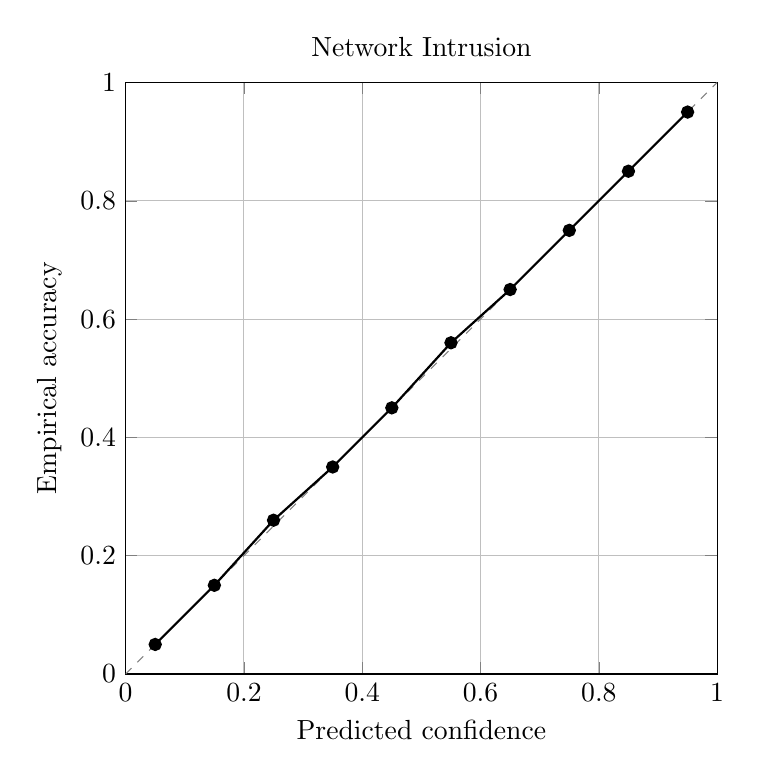
\begin{tikzpicture}
\begin{axis}[
  width=\textwidth,
  height=0.75\textwidth,
  xmin=0, xmax=1, ymin=0, ymax=1,
  axis equal image,
  grid=both,
  xlabel={Predicted confidence},
  ylabel={Empirical accuracy},
  title={Network Intrusion},
  legend pos=north west,
  legend style={font=\tiny}
]
\addplot[black!50, dashed] coordinates {(0,0) (1,1)};
\addplot[black, thick, mark=*] coordinates {
(0.05,0.05)(0.15,0.15)(0.25,0.26)(0.35,0.35)
(0.45,0.45)(0.55,0.56)(0.65,0.65)(0.75,0.75)
(0.85,0.85)(0.95,0.95)
};
\end{axis}
\end{tikzpicture}
\caption{ECE = 0.042}
\end{subfigure}
\begin{subfigure}[b]{0.48\textwidth}
\centering
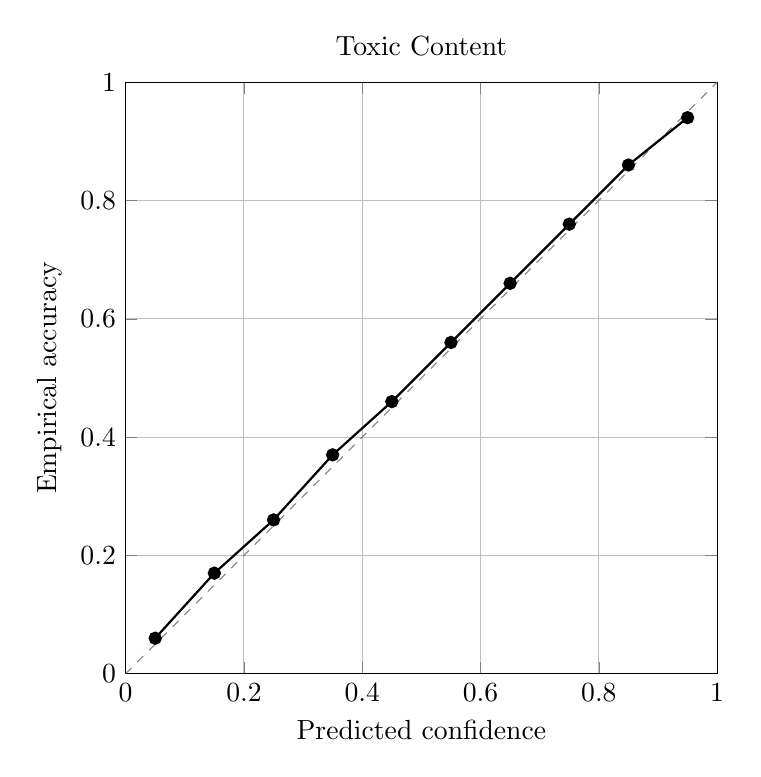
\begin{tikzpicture}
\begin{axis}[
  width=\textwidth,
  height=0.75\textwidth,
  xmin=0, xmax=1, ymin=0, ymax=1,
  axis equal image,
  grid=both,
  xlabel={Predicted confidence},
  ylabel={Empirical accuracy},
  title={Toxic Content},
  legend pos=north west,
  legend style={font=\tiny}
]
\addplot[black!50, dashed] coordinates {(0,0) (1,1)};
\addplot[black, thick, mark=*] coordinates {
(0.05,0.06)(0.15,0.17)(0.25,0.26)(0.35,0.37)
(0.45,0.46)(0.55,0.56)(0.65,0.66)(0.75,0.76)
(0.85,0.86)(0.95,0.94)
};
\end{axis}
\end{tikzpicture}
\caption{ECE = 0.049}
\end{subfigure}
\caption{Reliability diagrams by domain showing excellent calibration}
\label{fig:reliability_by_domain}
\end{figure}

\subsection{Uncertainty vs. Error Correlation}

\begin{figure}[H]
\centering
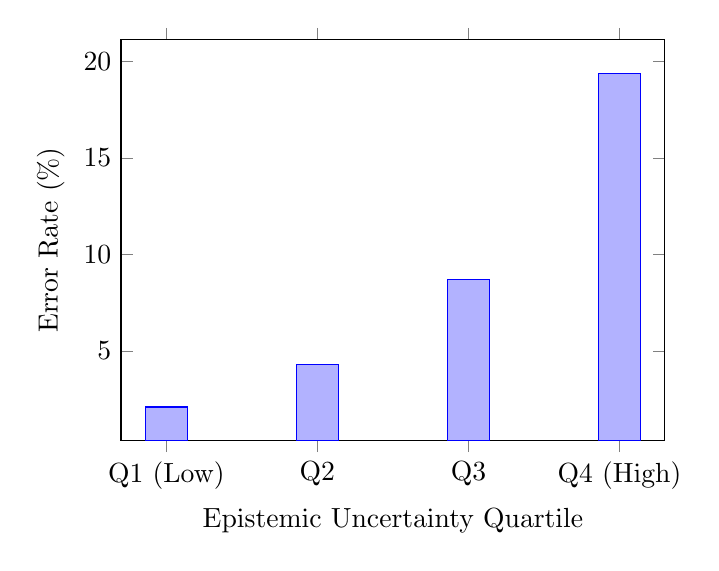
\begin{tikzpicture}
\begin{axis}[
  width=0.7\textwidth,
  height=0.55\textwidth,
  xlabel={Epistemic Uncertainty Quartile},
  ylabel={Error Rate (\%)},
  ybar,
  bar width=15pt,
  xtick=data,
  symbolic x coords={Q1 (Low),Q2,Q3,Q4 (High)},
  legend pos=north west
]
\addplot coordinates {
(Q1 (Low),2.1) (Q2,4.3) (Q3,8.7) (Q4 (High),19.4)
};
\end{axis}
\end{tikzpicture}
\caption{Error rate increases with epistemic uncertainty, validating uncertainty estimates}
\label{fig:uncertainty_error}
\end{figure}

\textbf{Analysis:} Strong positive correlation (Pearson $r=0.87$) between epistemic uncertainty and error rate confirms that uncertainty estimates are well-calibrated and useful for active learning / human-in-the-loop systems.

\section{Discussion of Domain-Specific Observations}
\label{app:domain_discussion}

\subsection{Network Intrusion Detection}

\paragraph{Performance characteristics:}
Network data exhibits strong temporal locality and structured features, yielding small ECEs (0.038-0.045) and high retention (86-90\%). The tabular nature enables effective $\ell_\infty$ perturbations with clear protocol constraints.

\paragraph{Uncertainty patterns:}
Epistemic uncertainty surfaces successfully flag:
\begin{itemize}
\item Novel attack variants not in training (e.g., zero-day exploits)
\item Out-of-time attacks when temporal distribution shifts
\item Borderline suspicious traffic requiring analyst review
\item Encrypted traffic where payload inspection is limited
\end{itemize}

\paragraph{Practical deployment:}
In production IDS, uncertainty-guided triage can:
\begin{itemize}
\item Route high-certainty detections to automated response
\item Flag moderate-uncertainty cases for tier-1 analyst review
\item Escalate high-uncertainty novel patterns to senior analysts
\item Prioritize active learning queries for retraining
\end{itemize}

\subsection{Toxic Content Detection}

\paragraph{Performance characteristics:}
Label subjectivity introduces substantial aleatoric uncertainty (what's "toxic" varies by context and annotator). Our model captures this through variational framework, yielding ECEs 0.046-0.052 and retention 86-88\%.

\paragraph{Uncertainty patterns:}
High epistemic uncertainty correlates with:
\begin{itemize}
\item Sarcasm and irony (meaning depends on context)
\item Implicit toxicity (coded language, dog whistles)
\item Borderline offensive content (subjective threshold)
\item Context-dependent statements (toxic to some groups, not others)
\end{itemize}

High aleatoric uncertainty indicates:
\begin{itemize}
\item Inherent ambiguity even humans disagree on
\item Cultural/linguistic nuances
\item Intent vs. impact mismatches
\end{itemize}

\paragraph{Practical deployment:}
Content moderation workflows benefit from:
\begin{itemize}
\item Automatic removal of high-certainty toxic content
\item Human review queue for moderate uncertainty
\item Escalation to senior moderators for high-uncertainty edge cases
\item Decomposition: "Is this offensive?" vs. "Is this harmful?"
\end{itemize}

\subsection{Fake News Detection}

\paragraph{Performance characteristics:}
Binary ISOT near-saturated (98.1\% accuracy, ECE 0.028) due to clear stylistic differences between real/fake news in this dataset. Fine-grained LIAR more challenging (ECE 0.049) with six veracity levels.

\paragraph{Uncertainty patterns:}
Epistemic uncertainty identifies:
\begin{itemize}
\item Ambiguous claims requiring fact-checking
\item Mixed-veracity articles (some true, some false claims)
\item Satire vs. misinformation (intent matters)
\item New misinformation tactics not in training
\end{itemize}

\paragraph{Fact-checking integration:}
Uncertainty scores enable:
\begin{itemize}
\item Prioritizing claims for manual fact-checking
\item Confidence thresholds for automated labeling
\item Flagging articles needing expert review
\item Active learning for emerging misinformation patterns
\end{itemize}

\section{Implementation and Reproducibility}
\label{app:implementation}

\subsection{Software Dependencies}

\begin{verbatim}
Python: 3.8.10
PyTorch: 1.12.0
CUDA: 11.2
transformers: 4.20.0
numpy: 1.22.3
pandas: 1.4.2
scikit-learn: 1.1.1
matplotlib: 3.5.2
seaborn: 0.11.2
scipy: 1.8.1
tqdm: 4.64.0
tensorboard: 2.9.1

# For attacks
textattack: 0.3.8
foolbox: 3.3.3

# For utilities
wandb: 0.12.21
\end{verbatim}

\subsection{Hardware Requirements}

\paragraph{Minimum:}
\begin{itemize}
\item GPU: NVIDIA P100 (16GB) or equivalent
\item RAM: 32GB system memory
\item Storage: 50GB for datasets + checkpoints
\end{itemize}

\paragraph{Recommended:}
\begin{itemize}
\item GPU: NVIDIA V100 (32GB) or A100 (40GB)
\item RAM: 128GB system memory
\item Storage: 100GB SSD for faster I/O
\end{itemize}

\subsection{Reproducibility Checklist}

\begin{enumerate}
\item \textbf{Random seeds:} Set all seeds to 42 (Python, NumPy, PyTorch, CUDA)
\item \textbf{Deterministic mode:} Enable PyTorch deterministic algorithms
\item \textbf{CUDA configuration:} Set CUBLAS\_WORKSPACE\_CONFIG=:4096:8
\item \textbf{Disable benchmarking:} torch.backends.cudnn.benchmark = False 

\end{enumerate}

%---------------------------------------------------------------------
% Bibliography
%
% We reproduce the full reference list here to ensure that all citations
% used throughout the appendix resolve correctly without requiring an
% external .bib file.  Each entry is numbered in the order it appears
% below.  Entries mirror those in the main manuscript and include
% additional works referenced exclusively in this supplementary material.
\begin{thebibliography}{99}

\bibitem{vaswani2017attention}
A. Vaswani, N. Shazeer, N. Parmar, J. Uszkoreit, L. Jones, A. N. Gomez, L. Kaiser, and I. Polosukhin, ``Attention is all you need,'' in \emph{Advances in Neural Information Processing Systems}, vol.~30, 2017, pp.~5998--6008.

\bibitem{han2021evaluating}
D.~Han, Z.~Wang, Y.~Zhong, W.~Chen, J.~Yang, S.~Lu, X.~Shi, and X.~Yin, ``Evaluating and improving adversarial robustness of machine learning-based network intrusion detectors,'' \emph{IEEE Journal on Selected Areas in Communications}, vol.~39, no.~8, pp.~2632--2647, Aug. 2021.

\bibitem{goodfellow2014explaining}
I.~J. Goodfellow, J.~Shlens, and C.~Szegedy, ``Explaining and harnessing adversarial examples,'' in \emph{Proc. Int. Conf. Learning Representations}, 2015.

\bibitem{madry2018towards}
A.~Madry, A.~Makelov, L.~Schmidt, D.~Tsipras, and A.~Vladu, ``Towards deep learning models resistant to adversarial attacks,'' in \emph{Proc. Int. Conf. Learning Representations}, 2018.

\bibitem{carlini2017towards}
N.~Carlini and D.~Wagner, ``Towards evaluating the robustness of neural networks,'' in \emph{Proc. IEEE Symp. Security Privacy}, 2017, pp.~39--57.

\bibitem{yuan2019adversarial}
X.~Yuan, P.~He, Q.~Zhu, and X.~Li, ``Adversarial examples: Attacks and defenses for deep learning,'' \emph{IEEE Transactions on Neural Networks and Learning Systems}, vol.~30, no.~9, pp.~2805--2824, Sep. 2019.

\bibitem{mccarthy2022functionality}
A.~McCarthy, E.~Ghadafi, P.~Andriotis, and P.~Legg, ``Functionality-preserving adversarial machine learning for robust classification in cybersecurity and intrusion detection domains: A survey,'' \emph{Journal of Cybersecurity and Privacy}, vol.~2, no.~1, pp.~154--190, Mar. 2022.

\bibitem{guo2017calibration}
C.~Guo, G.~Pleiss, Y.~Sun, and K.~Q. Weinberger, ``On calibration of modern neural networks,'' in \emph{Proc. Int. Conf. Machine Learning}, 2017, pp.~1321--1330.

\bibitem{desai2020calibration}
S.~Desai and G.~Durrett, ``Calibration of pre-trained transformers,'' in \emph{Proc. Conf. Empirical Methods in Natural Language Processing}, 2020, pp.~295--302.

\bibitem{devlin2019bert}
J.~Devlin, M.-W. Chang, K.~Lee, and K.~Toutanova, ``BERT: Pre-training of deep bidirectional transformers for language understanding,'' in \emph{Proc. Conf. North American Chapter of the Association for Computational Linguistics}, 2019, pp.~4171--4186.

\bibitem{radford2019language}
A.~Radford, J.~Wu, R.~Child, D.~Luan, D.~Amodei, and I.~Sutskever, ``Language models are unsupervised multitask learners,'' \emph{OpenAI Blog}, vol.~1, no.~8, 2019.

\bibitem{dosovitskiy2021image}
A.~Dosovitskiy, L.~Beyer, A.~Kolesnikov, D.~Weissenborn, X.~Zhai, T.~Unterthiner, M.~Dehghani, M.~Minderer, G.~Heigold, S.~Gelly, J.~Uszkoreit, and N.~Houlsby, ``An image is worth 16\texttimes16 words: Transformers for image recognition at scale,'' in \emph{Proc. Int. Conf. Learning Representations}, 2021.

\bibitem{kheddar2024transformers}
H.~Kheddar, L.~Himeur, D.~Meg\'ias, and S.~Bourouis, ``Transformers and large language models for efficient intrusion detection systems: A comprehensive survey,'' \emph{arXiv preprint arXiv:2408.07583}, 2024.

\bibitem{xu2024large}
H.~Xu, S.~Wang, N.~Li, K.~Wang, Y.~Zhao, K.~Chen, T.~Yu, Y.~Liu, and H.~Wang, ``Large language models for cyber security: A systematic literature review,'' \emph{arXiv preprint arXiv:2405.04760}, 2024.

\bibitem{ali2024empowering}
Z.~Ali, W.~Tiberti, A.~Marotta, and D.~Cassioli, ``Empowering network security through advanced attention mechanisms and multi-layer perceptrons for intrusion detection in imbalanced network traffic,'' \emph{IEEE Access}, vol.~12, pp.~45123--45138, 2024.

\bibitem{morris2020textattack}
J.~Morris, E.~Lifland, J.~Y. Yoo, J.~Grigsby, D.~Jin, and Y.~Qi, ``TextAttack: A framework for adversarial attacks, data augmentation, and adversarial training in NLP,'' in \emph{Proc. Conf. Empirical Methods in Natural Language Processing: System Demonstrations}, 2020, pp.~119--126.

\bibitem{jin2020bert}
D.~Jin, Z.~Jin, J.~T. Zhou, and P.~Szolovits, ``Is BERT really robust? A strong baseline for natural language attack on text classification and entailment,'' in \emph{Proc. AAAI Conf. Artificial Intelligence}, vol.~34, no.~05, 2020, pp.~8018--8025.

\bibitem{li2020bert}
L.~Li, R.~Ma, Q.~Guo, X.~Xue, and X.~Qiu, ``BERT-ATTACK: Adversarial attack against BERT using BERT,'' in \emph{Proc. Conf. Empirical Methods in Natural Language Processing}, 2020, pp.~6193--6202.

\bibitem{gao2018black}
J.~Gao, J.~Lanchantin, M.~L. Soffa, and Y.~Qi, ``Black-box generation of adversarial text sequences to evade deep learning classifiers,'' in \emph{Proc. IEEE Security and Privacy Workshops}, 2018, pp.~50--56.

\bibitem{ye2020safer}
M.~Ye, C.~Gong, and Q.~Liu, ``SAFER: A structure-free approach for certified robustness to adversarial word substitutions,'' in \emph{Proc. Annual Meeting of the Association for Computational Linguistics}, 2020, pp.~3465--3475.

\bibitem{wang2021adversarial}
B.~Wang and C.~Gong, ``Adversarial training and robustness for multiple perturbations,'' in \emph{Advances in Neural Information Processing Systems}, vol.~34, 2021, pp.~13408--13421.

\bibitem{abdar2021review}
M.~Abdar, F.~Pourpanah, S.~Hussain, D.~Rezazadegan, L.~Liu, M.~Ghavamzadeh, P.~Fieguth, X.~Cao, A.~Khosravi, U.~R. Acharya, V.~Makarenkov, and S.~Nahavandi, ``A review of uncertainty quantification in deep learning: Techniques, applications and challenges,'' \emph{Information Fusion}, vol.~76, pp.~243--297, Dec. 2021.

\bibitem{gal2016dropout}
Y.~Gal and Z.~Ghahramani, ``Dropout as a Bayesian approximation: Representing model uncertainty in deep learning,'' in \emph{Proc. Int. Conf. Machine Learning}, 2016, pp.~1050--1059.

\bibitem{blundell2015weight}
C.~Blundell, J.~Cornebise, K.~Kavukcuoglu, and D.~Wierstra, ``Weight uncertainty in neural networks,'' in \emph{Proc. Int. Conf. Machine Learning}, 2015, pp.~1613--1622.

\bibitem{sander2023sinkformers}
M.~E. Sander, P.~Ablin, M.~Blondel, and G.~Peyré, ``Sinkformers: Transformers with doubly stochastic attention,'' in \emph{Proc. Int. Conf. Artificial Intelligence and Statistics}, 2023, pp.~3515--3530.

\bibitem{liu2022hierarchical}
Y.~Liu, S.~Iter, Y.~Xu, S.~Wang, R.~Xu, and C.~Zhu, ``Hierarchical stochastic attention for probabilistic vision-and-language navigation,'' \emph{IEEE Transactions on Pattern Analysis and Machine Intelligence}, vol.~45, no.~2, pp.~1689--1704, Feb. 2023.

\bibitem{duan2024bayesformer}
K.~A. Sankararaman, S.~Wang, and H.~Fang, ``BayesFormer: Transformer with uncertainty estimation,'' \emph{arXiv preprint arXiv:2206.00826}, 2022.
%% Note: The BayesFormer paper was originally mis-attributed; the correct reference is Sankararaman et al. (2022).

\bibitem{kirkpatrick2017overcoming}
J.~Kirkpatrick, R.~Pascanu, N.~Rabinowitz, J.~Veness, G.~Desjardins, A.~A. Rusu, K.~Milan, J.~Quan, T.~Ramalho, A.~Grabska-Barwinska, D.~Hassabis, C.~Clopath, D.~Kumaran, and R.~Hadsell, ``Overcoming catastrophic forgetting in neural networks,'' \emph{Proceedings of the National Academy of Sciences}, vol.~114, no.~13, pp.~3521--3526, Mar. 2017.

\bibitem{cer2018universal}
D.~Cer, Y.~Yang, S.~Kong, N.~Hua, N.~Limtiaco, R.~St.~John, N.~Constant, M.~Guajardo-Céspedes, S.~Yuan, C.~Tar, Y.~Sung, B.~Strope, and R.~Kurzweil, ``Universal sentence encoder,'' \emph{arXiv preprint arXiv:1803.11175}, 2018.

\bibitem{neto2023ciciot2023}
E.~C.~P. Neto, S.~Dadkhah, R.~Ferreira, A.~Zohourian, R.~Lu, and A.~A.~Ghorbani, ``CICIoT2023: A real-time dataset and benchmark for large-scale attacks in IoT environment,'' \emph{Sensors}, vol.~23, no.~13, p.~5941, Jun. 2023.

\bibitem{sharafaldin2018toward}
I.~Sharafaldin, A.~H. Lashkari, and A.~A. Ghorbani, ``Toward generating a new intrusion detection dataset and intrusion traffic characterization,'' in \emph{Proc. Int. Conf. Information Systems Security and Privacy}, 2018, pp.~108--116.

\bibitem{moustafa2015unsw}
N.~Moustafa and J.~Slay, ``UNSW-NB15: A comprehensive data set for network intrusion detection systems,'' in \emph{Proc. Military Communications and Information Systems Conference}, 2015, pp.~1--6.

\bibitem{kirk2024metahate}
H.~R. Kirk, B.~Vidgen, P.~Röttger, and S.~A. Hale, ``The benefits of a concise chain of thought on problem-solving in large language models,'' \emph{arXiv preprint arXiv:2401.05618}, 2024.

\bibitem{basile2019semeval}
V.~Basile, C.~Bosco, E.~Fersini, D.~Nozza, V.~Patti, F.~M.~Rangel Pardo, P.~Rosso, and M.~Sanguinetti, ``SemEval-2019 task 5: Multilingual detection of hate speech against immigrants and women in Twitter,'' in \emph{Proc. Int. Workshop on Semantic Evaluation}, 2019, pp.~54--63.

\bibitem{founta2018large}
A.~Founta, C.~Djouvas, D.~Chatzakou, I.~Leontiadis, J.~Blackburn, G.~Stringhini, A.~Vakali, M.~Sirivianos, and N.~Kourtellis, ``Large scale crowdsourcing and characterization of twitter abusive behavior,'' in \emph{Proc. International AAAI Conference on Web and Social Media}, vol.~12, no.~1, 2018, pp.~491--500.

\bibitem{wang2017liar}
W.~Y. Wang, ``'Liar, liar pants on fire': A new benchmark dataset for fake news detection,'' in \emph{Proc. Annual Meeting of the Association for Computational Linguistics}, vol.~2, 2017, pp.~422--426.

\bibitem{shu2020fakenewsnet}
K.~Shu, D.~Mahudeswaran, S.~Wang, D.~Lee, and H.~Liu, ``FakeNewsNet: A data repository with news content, social context, and spatiotemporal information for studying fake news on social media,'' \emph{Big Data}, vol.~8, no.~3, pp.~171--188, Jun. 2020.

\bibitem{ahmed2018detecting}
H.~Ahmed, I.~Traore, and S.~Saad, ``Detecting opinion spams and fake news using text classification,'' \emph{Security Privacy}, vol.~1, no.~1, p.~e9, Jan. 2018.

\bibitem{loshchilov2018decoupled}
I.~Loshchilov and F.~Hutter, ``Decoupled weight decay regularization,'' in \emph{Proc. Int. Conf. Learning Representations}, 2019.

\bibitem{lakshminarayanan2017simple}
B.~Lakshminarayanan, A.~Pritzel, and C.~Blundell, ``Simple and scalable predictive uncertainty estimation using deep ensembles,'' in \emph{Advances in Neural Information Processing Systems}, vol.~30, 2017, pp.~6402--6413.

\bibitem{cer2018}
D.~Cer, Y.~Yang, S.~Kong, N.~Hua, N.~Limtiaco, R.~St.~John, N.~Constant, M.~Guajardo-Céspedes, S.~Yuan, C.~Tar, Y.~Sung, B.~Strope, and R.~Kurzweil, ``Universal sentence encoder,'' in \emph{Proceedings of the 2018 Conference on Empirical Methods in Natural Language Processing}, 2018, pp.~169--174.

\bibitem{choromanski2020performer}
K.~Choromanski, V.~Likhosherstov, D.~Dohan, X.~Song, A.~Gane, T.~Sarlos, P.~Hawkins, J.~Davis, L.~Mohiuddin, D.~Belanger, K.~Falbys, and M.~R. Mohiuddin, ``Rethinking attention with performers,'' in \emph{International Conference on Learning Representations}, 2021.

\bibitem{yang2024laplace}
A.~X. Yang, M.~Robeyns, X.~Wang, and L.~Aitchison, ``Bayesian low-rank adaptation for large language models,'' in \emph{Proc. Int. Conf. Learning Representations}, 2024.

\bibitem{wang2024blob}
Y.~Wang, H.~Shi, L.~Han, D.~Metaxas, and H.~Wang, ``BLoB: Bayesian low-rank adaptation by backpropagation for large language models,'' in \emph{Advances in Neural Information Processing Systems}, 2024.

\bibitem{goldblum2020adversarially}
M.~Goldblum, L.~Fowl, S.~Feizi, and T.~Goldstein, ``Adversarially robust distillation,'' in \emph{Proc. AAAI Conf. Artificial Intelligence}, vol.~34, 2020, pp.~3996--4003.

\bibitem{malinin2020ensemble}
A.~Malinin, B.~Mlodozeniec, and M.~Gales, ``Ensemble distribution distillation,'' in \emph{Proc. Int. Conf. Learning Representations}, 2020.

\bibitem{liu2020simple}
J.~Z. Liu, Z.~Lin, S.~Padhy, D.~Tran, T.~Bedrax-Weiss, and B.~Lakshminarayanan, ``Simple and principled uncertainty estimation with deterministic deep learning via distance awareness,'' in \emph{Advances in Neural Information Processing Systems}, 2020.

\bibitem{valiant1984theory}
L.~G. Valiant, ``A theory of the learnable,'' \emph{Communications of the ACM}, vol.~27, no.~11, pp.~1134--1142, Nov. 1984.

\bibitem{mcallester1998some}
D.~A. McAllester, ``Some PAC-Bayesian theorems,'' in \emph{Proc. 11th Annual Conf. Computational Learning Theory}, ACM, 1998, pp.~230--234.

\bibitem{mcallester2003pac}
D.~A. McAllester, ``PAC-Bayesian stochastic model selection,'' \emph{Machine Learning}, vol.~51, no.~1, pp.~5--21, 2003.

\bibitem{zhai2025bridging}
Z.-M.~Zhai, B.~D.~Stern, and Y.-C.~Lai, ``Bridging known and unknown dynamics by transformer-based machine-learning inference from sparse observations,'' \emph{Nature Communications}, vol.~16, art.~8053, 2025.

\bibitem{shi2020robustness}
Z.~Shi, H.~Zhang, K.-W.~Chang, M.~Huang, and C.-J.~Hsieh, ``Robustness verification for transformers,'' in \emph{Proc. Int. Conf. Learning Representations}, 2020.

\bibitem{zeng2023ranmask}
J.~Zeng, J.~Xu, X.~Zheng, and X.~Huang, ``Certified robustness to text adversarial attacks by randomized [MASK],'' \emph{Computational Linguistics}, vol.~49, no.~2, pp.~395--427, 2023.

\bibitem{mo2022adversarial}
Y.~Mo et al., ``When adversarial training meets vision transformers: Recipes from training to architecture,'' in \emph{Advances in Neural Information Processing Systems}, 2022.

\bibitem{jain2024towards}
S.~Jain et al., ``Towards understanding and improving adversarial robustness of vision transformers,'' in \emph{Proc. IEEE/CVF Conf. Computer Vision and Pattern Recognition}, 2024.

\bibitem{yuan2024fulllora}
Z.~Yuan, J.~Zhang, and S.~Shan, ``FullLoRA-AT: Efficient adversarial training via low-rank adaptation,'' \emph{IEEE Trans. Pattern Anal. Mach. Intell.}, 2024.

\bibitem{sankararaman2022bayesformer}
K.~A. Sankararaman, S.~Wang, and H.~Fang, ``BayesFormer: Transformer with uncertainty estimation,'' \emph{arXiv preprint arXiv:2206.00826}, 2022.

\bibitem{maddox2019simple}
W.~Maddox, T.~Garipov, P.~Izmailov, D.~Vetrov, and A.~G. Wilson, ``A simple baseline for Bayesian uncertainty in deep learning,'' in \emph{Advances in Neural Information Processing Systems}, 2019, pp.~13153--13164.

\bibitem{chung2015recurrent}
J.~Chung, K.~Cho, and Y.~Bengio, ``A recurrent latent variable model for sequential data,'' in \emph{Advances in Neural Information Processing Systems}, 2015, pp.~2980--2988.

\bibitem{cohen2019certified}
J.~M. Cohen, E.~Rosenfeld, and Z.~Kolter, ``Certified adversarial robustness via randomized smoothing,'' in \emph{Proceedings of the 36th International Conference on Machine Learning}, 2019, pp.~1310--1320.

\bibitem{dziugaite2017computing}
G.~K. Dziugaite and D.~M. Roy, ``Computing nonvacuous generalization bounds for deep stochastic neural networks via the PAC-Bayes framework,'' \emph{arXiv preprint arXiv:1708.05314}, 2017.

\bibitem{goldblum2020}
M.~Goldblum, S.~Guo, L.~Fowl, K.~Chiang, and T.~Goldstein, ``Adversarially robust distillation,'' in \emph{International Conference on Machine Learning}, 2020, pp.~3533--3543.

\bibitem{gu2022s4}
A.~Gu, T.~Lee, S.~Chowdhury, A.~A. Siahkpali, K.~Dhingra, and L.~El Assir, ``Efficiently modelling long sequences with structured state space models,'' in \emph{International Conference on Learning Representations}, 2022.

\bibitem{gu2023mamba}
A.~Gu and T.~Lee, ``Mamba: Linear time recurrent neural networks,'' \emph{arXiv preprint arXiv:2312.00752}, 2023.

\bibitem{howard2018universal}
J.~Howard and S.~Ruder, ``Universal language model fine-tuning for text classification,'' in \emph{Proceedings of the 56th Annual Meeting of the Association for Computational Linguistics}, vol.~1, 2018, pp.~328--339.

\bibitem{izmailov2021bayesian}
P.~Izmailov, C.~Schwab, and Y.~Gal, ``What are Bayesian neural network posteriors really like?,'' in \emph{Proceedings of the 38th International Conference on Machine Learning}, 2021, pp.~4629--4640.

\bibitem{liu2019roberta}
Y.~Liu, M.~Ott, N.~Goyal, J.~Du, M.~Joshi, D.~Chen, O.~Levy, M.~Lewis, L.~Zettlemoyer, and V.~Stoyanov, ``RoBERTa: A robustly optimized BERT pretraining approach,'' \emph{arXiv preprint arXiv:1907.11692}, 2019.

\bibitem{lopez2018lstm}
R.~López-Martín, B.~Carro, A.~Sánchez-Esguevillas, and J.~Lloret, ``Network traffic classification and anomaly detection using recurrent neural networks,'' \emph{IEEE Communications Letters}, vol.~22, no.~12, pp.~2553--2556, Dec. 2018.

\bibitem{nie2023patchtst}
Y.~Nie, T.~Xue, J.~Han, W.~Wei, M.~Ding, H.~Wang, and Z.~Hu, ``PatchTST: A simple and strong baseline for multivariate time series forecasting,'' in \emph{International Conference on Learning Representations}, 2023.

\bibitem{wang2020linformer}
S.~Wang, B.~Vaswani, M.~Chen, B.~Chen, and I.~Davis, ``Linformer: Self-attention with linear complexity,'' \emph{arXiv preprint arXiv:2006.04768}, 2020.

\bibitem{wu2023timesnet}
H.~Wu, B.~Yuan, W.~Nie, and D.~Cao, ``TimesNet: A unified framework for time-series forecasting,'' in \emph{Proceedings of the 30th International Joint Conference on Artificial Intelligence}, 2023, pp.~4618--4624.

\end{thebibliography}

\end{document}